\clearpage

\section {Sensitivity studies}
\label{sec:sensitivity}
To determine the sensitivity of the analysis a number of fits were performed using Asimov data sets A and B, the contours for which indicate the ability of the analysis to measure the oscillation parameters in the absence of statistical fluctuations and under the assumption that their true values correspond to the Asimov values. Fits of single parameters are performed for each of \ssqthonethree, \deltacp, \ssqthtwothree and \dmsq (\dmsqtwothree in normal hierarchy and \dmsqonethree in inverted hierarchy), with two-dimensional fits being performed for \appearance and \disappearance. Fits are performed for each of normal and inverted hierarchy, and also with and without the reactor constraint on \ssqthonethree.

\subsection{Results for Asimov sets A and B}
\label{sec:sensitivity:asimov_results}

\subsubsection{Results for \appearance}
In \cref{fig:ssqth13_vs_dcp_sensitivity} the sensitivity to \appearance with reactor constraint and T2K only is shown for the Asimov data sets A and B. Note that in the Asimov B case it can be seen that the best-fit point in inverted hierarchy is shifted away from the true \deltacp value of zero towards $-\pi$. In addition to best-fit points being moved from the true value due to marginalisation of oscillation and systematic parameters there are additional contributing effects. There is a lack of sensitivity to distinguish $\delta_{CP} = 0$ and $\delta_{CP} = \pi$ due to the spectra for $\delta_{CP} = 0$ in inverted hierarchy being similar to the spectra for $\delta_{CP} = \pi$ in normal hierarchy and vice versa (see \cref{fig:asimovb_spectra_degeneracy} in \cref{app:asimovb_sensitivity}), leading to similar $\Delta\chi^2$ values for the two points. This can be seen in \cref{fig:dcp_sensitivity}(c) and \cref{fig:dcp_sensitivity}(d), with the difference in $\Delta\chi^2_{true}$ and $\Delta\chi^2_{best-fit}$ being only $\sim 0.2$. Furthermore, degeneracy between \deltacp and mass hierarchy can cause $\delta_{CP} = 0$ to behave more like $\delta_{CP} = \pi/2$ in inverted hierarchy, and more like $\delta_{CP} = -\pi/2$ in normal hierarchy, shifting the best-fit for inverted hierarchy away from zero to a value between $-\pi$ and $-\pi/2$.

\begin{figure*}[htb]
	\center
	\begin{subfigure}[b]{0.49\textwidth}
		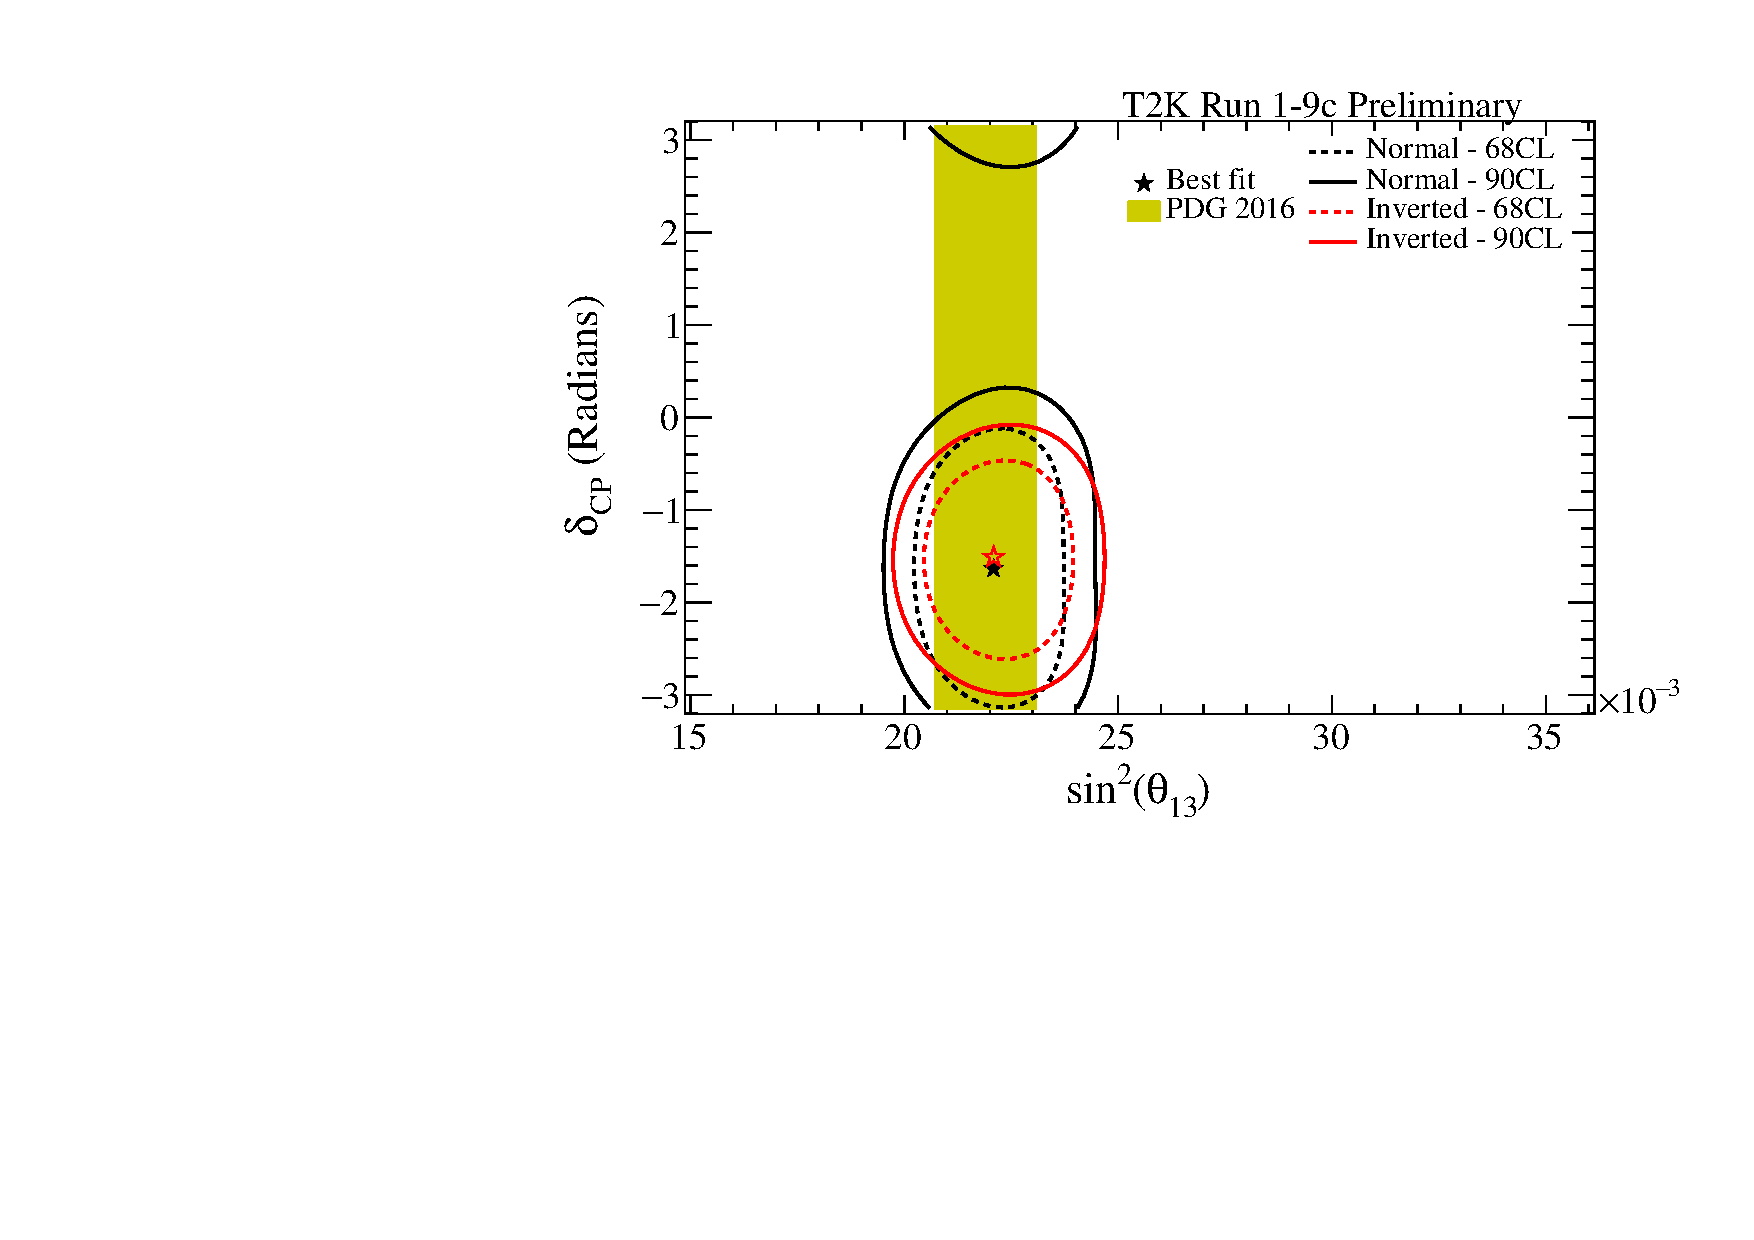
\includegraphics[width=0.9\textwidth]{images/sensitivity/mixing13_deltacp_AsimovA_reactor_global}
		\caption{Asimov A \appearance with reactor constraint}
	\end{subfigure}
	\begin{subfigure}[b]{0.49\textwidth}
		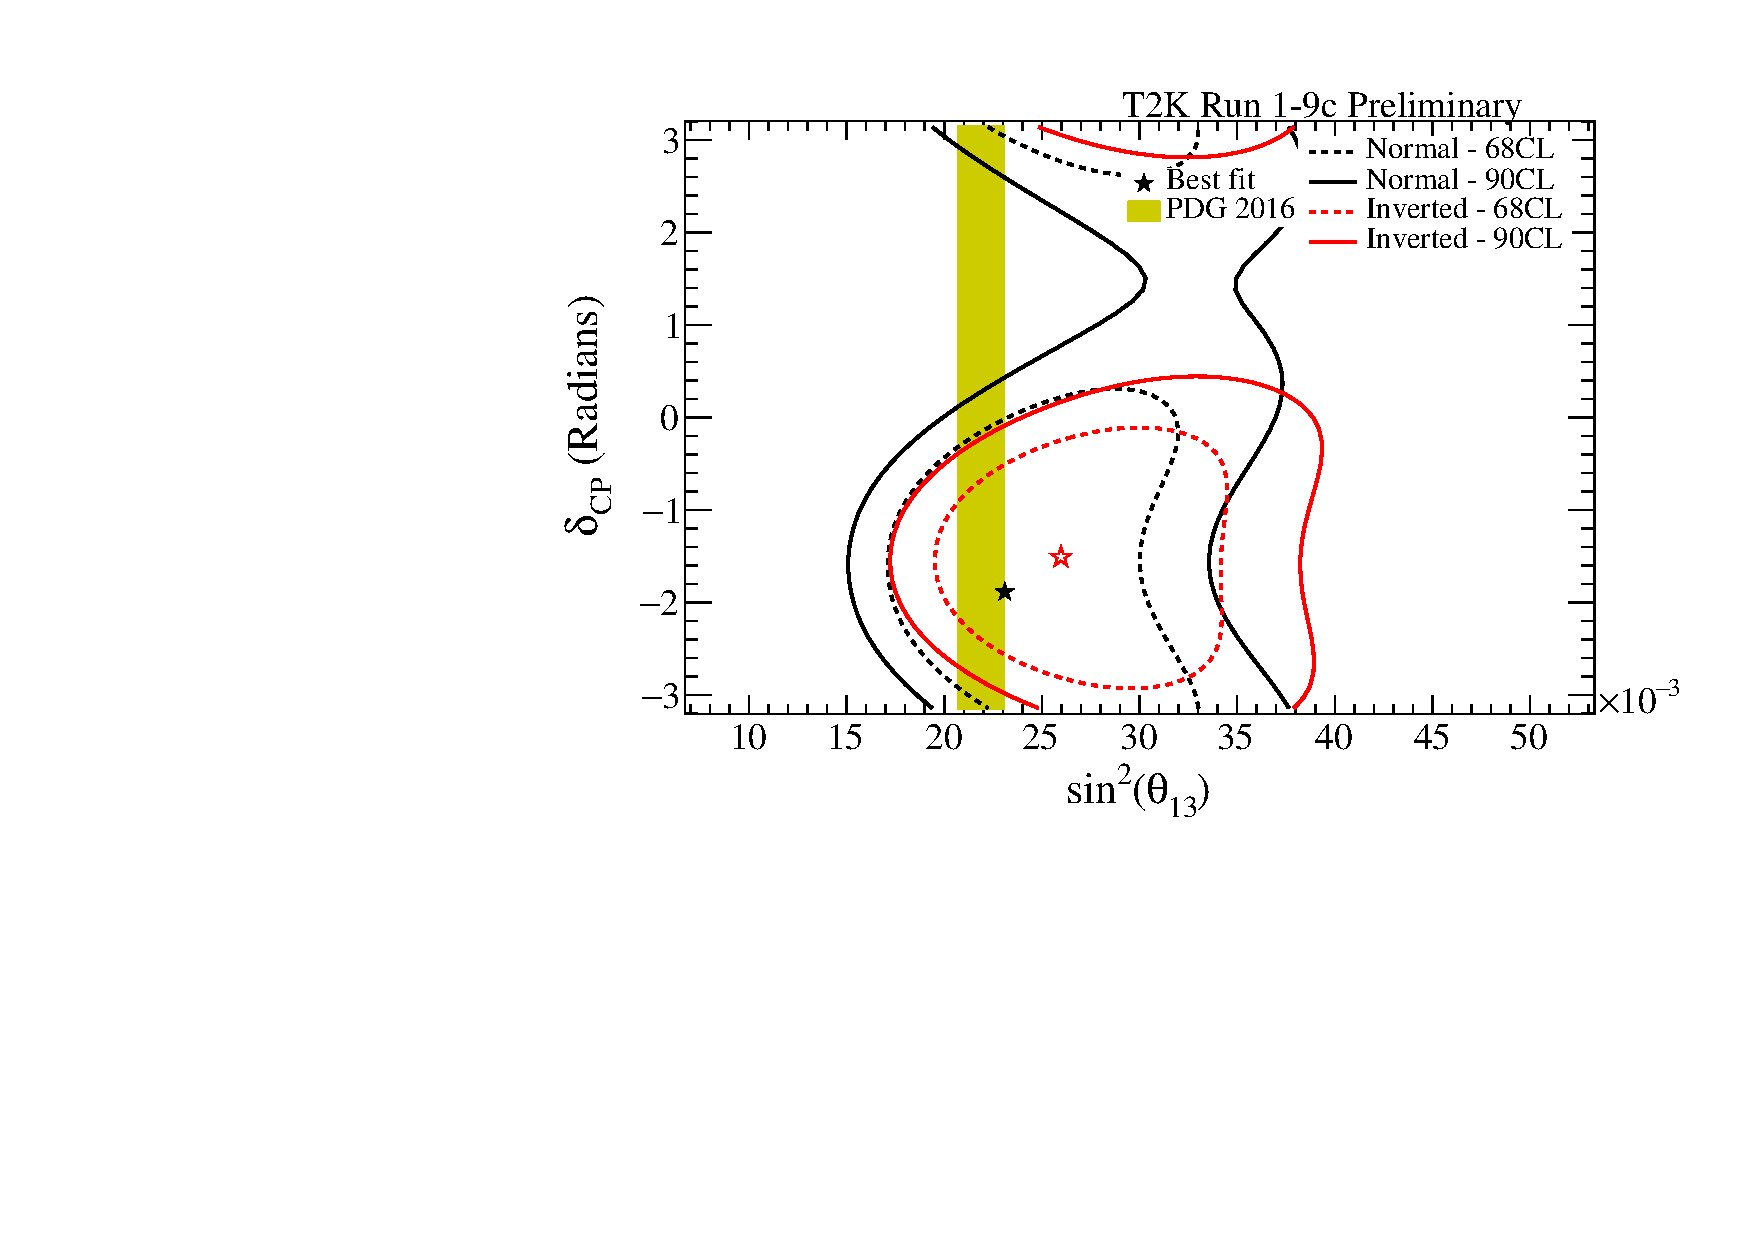
\includegraphics[width=0.9\textwidth]{images/sensitivity/mixing13_deltacp_AsimovA_t2k_global}
		\caption{Asimov A \appearance T2K only}
	\end{subfigure}
	\begin{subfigure}[b]{0.49\textwidth}
		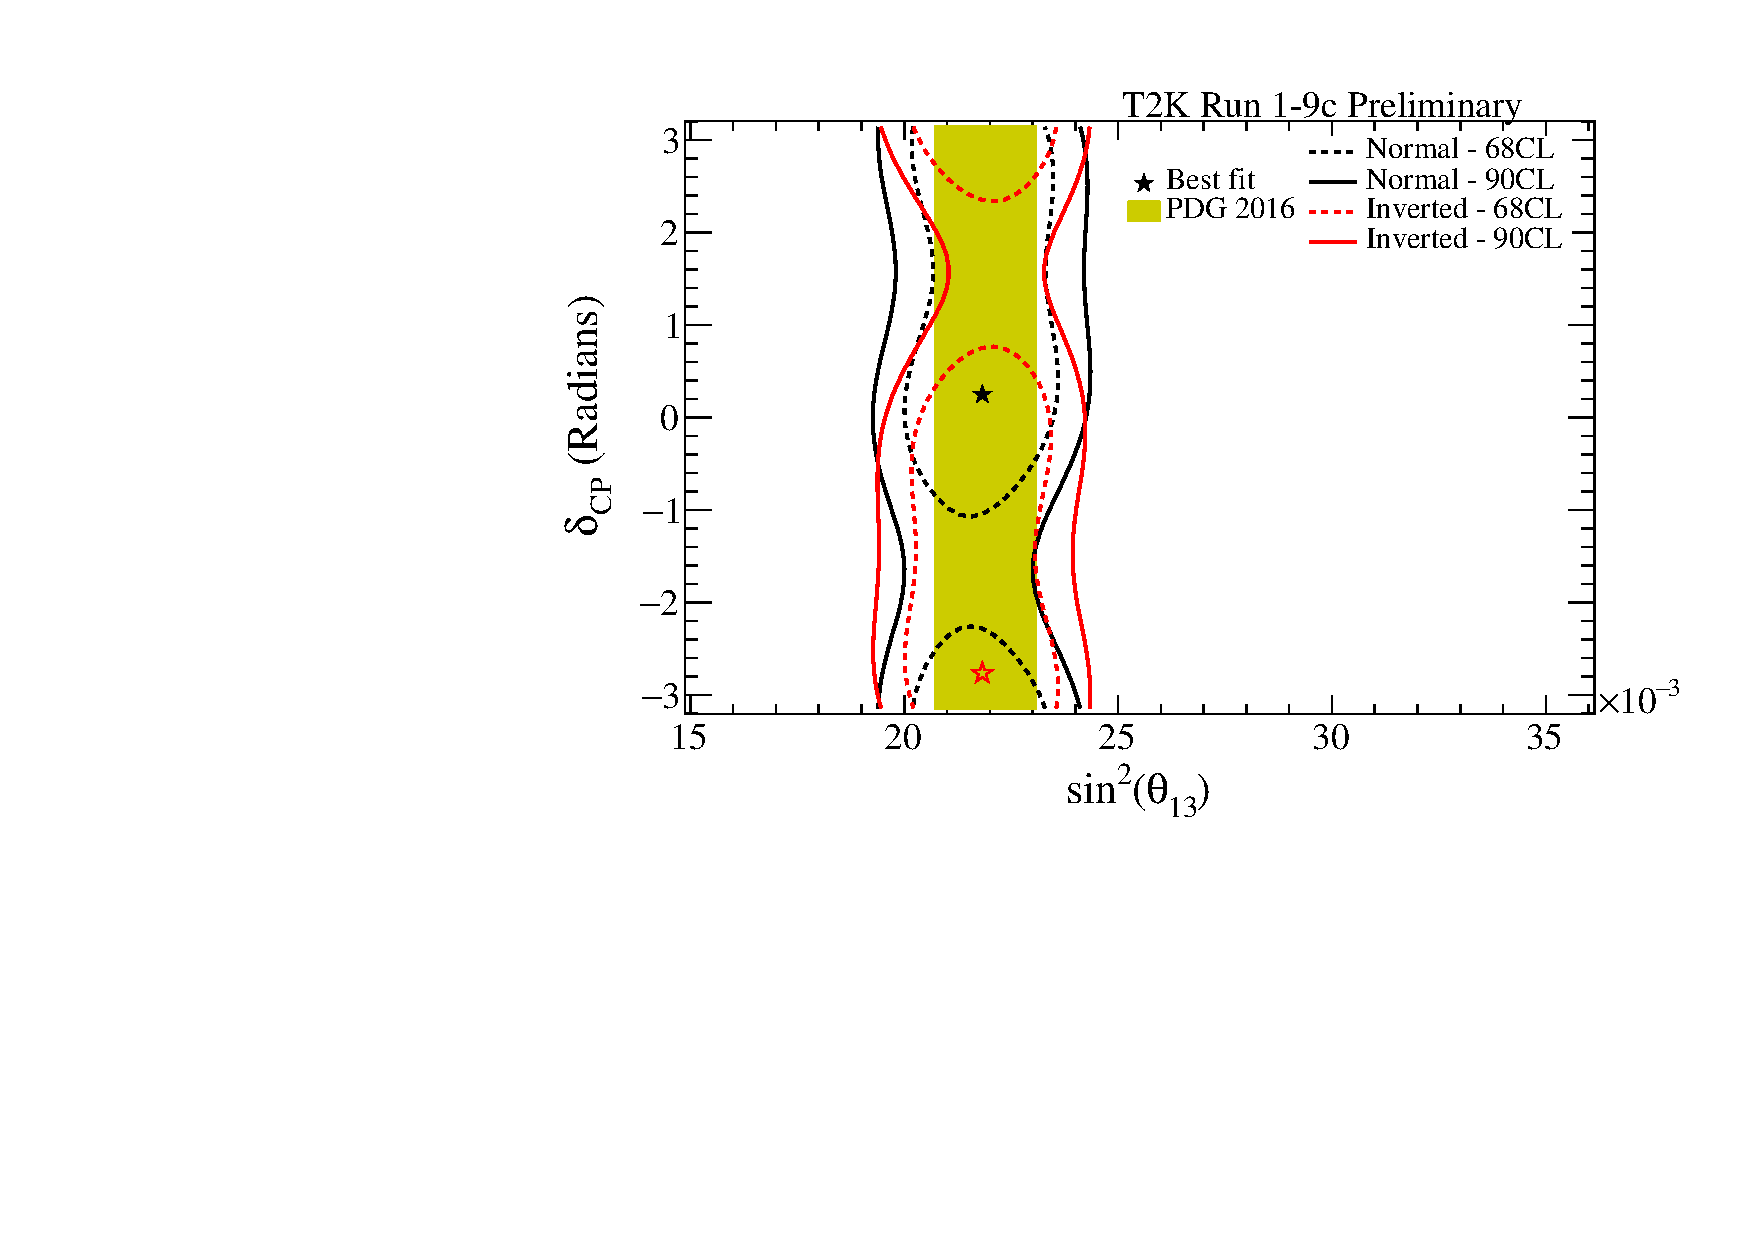
\includegraphics[width=0.9\textwidth]{images/sensitivity/mixing13_deltacp_AsimovB_reactor_global}
		\caption{Asimov B \appearance with reactor constraint}
	\end{subfigure}
	\begin{subfigure}[b]{0.49\textwidth}
		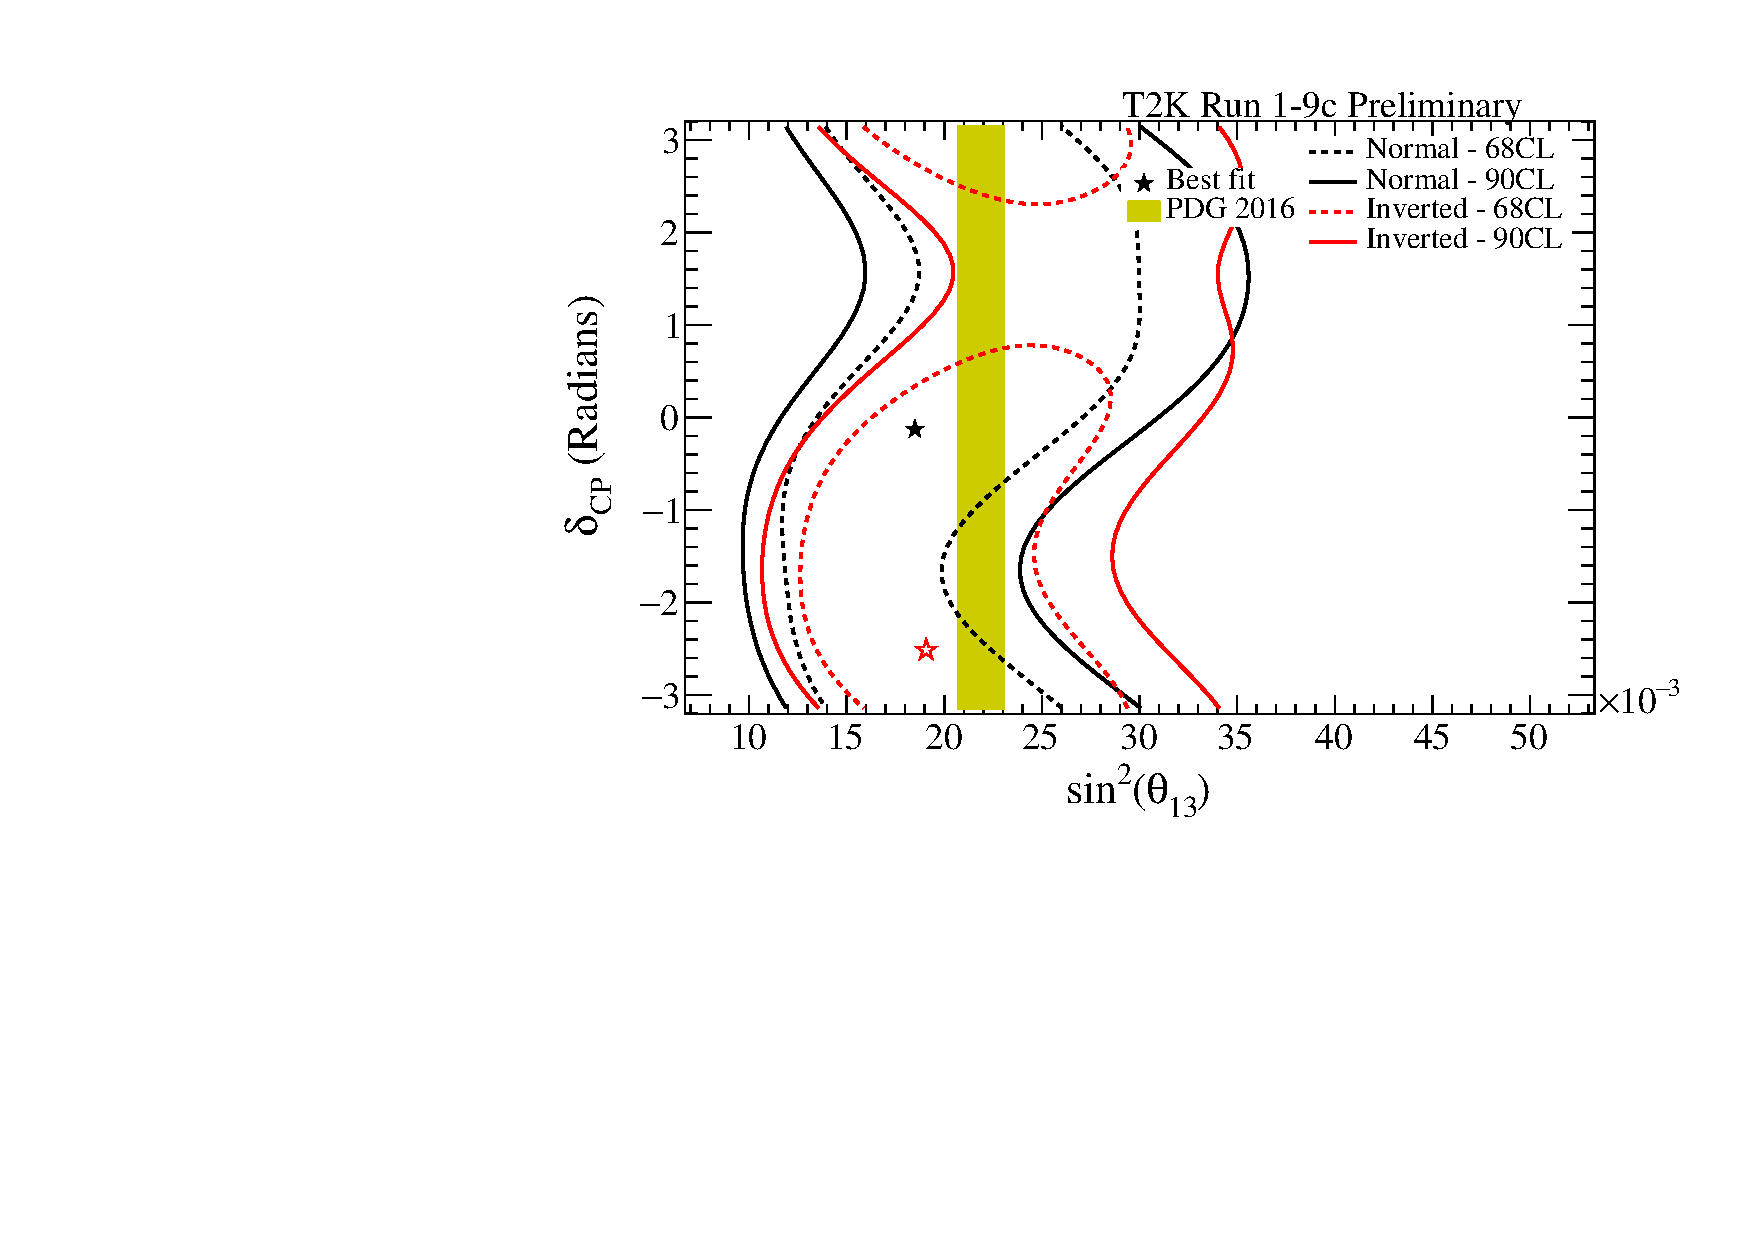
\includegraphics[width=0.9\textwidth]{images/sensitivity/mixing13_deltacp_AsimovB_t2k_global}
		\caption{Asimov B \appearance T2K only}
	\end{subfigure}
	\caption {
		Contours at 68\% and 90\% CL for \appearance with and without reactor constraint for Asimov data sets A and B. Normal and inverted hierarchy contours are independent. All 5 samples were used to produce these fits.
	}
	\label{fig:ssqth13_vs_dcp_sensitivity}
\end{figure*}
\clearpage
\subsubsection{Results for \disappearance}

The sensitivity to \disappearance with reactor constraint and T2K only is shown for the Asimov data sets A and B in fig.~\ref{fig:ssqth23_vs_dmsq23_sensitivity}.

\begin{figure*}[htb]
	\center
	\begin{subfigure}[b]{0.49\textwidth}
		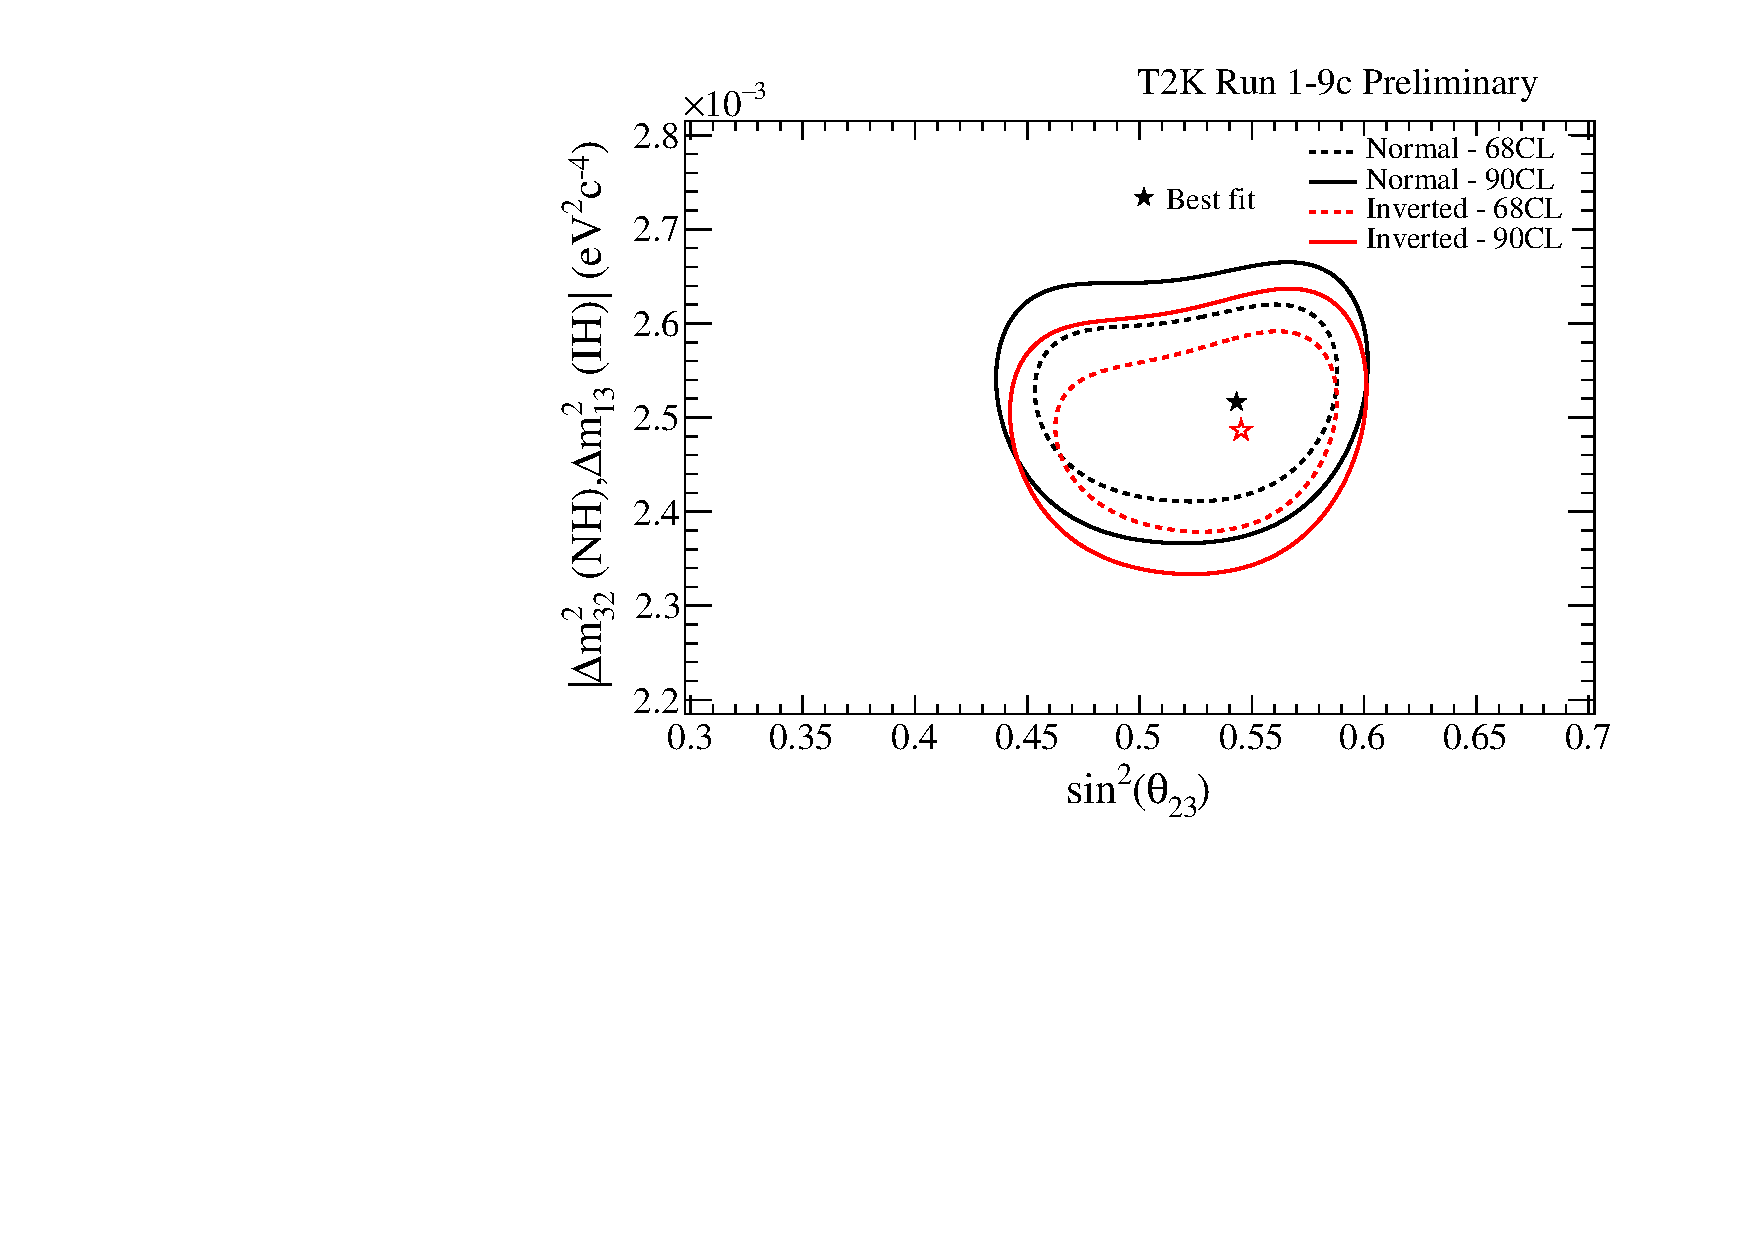
\includegraphics[width=0.9\textwidth]{images/sensitivity/mixing23_dmsq23_AsimovA_reactor_global}
		\caption{Asimov A \disappearance with reactor constraint}
	\end{subfigure}
	\begin{subfigure}[b]{0.49\textwidth}
		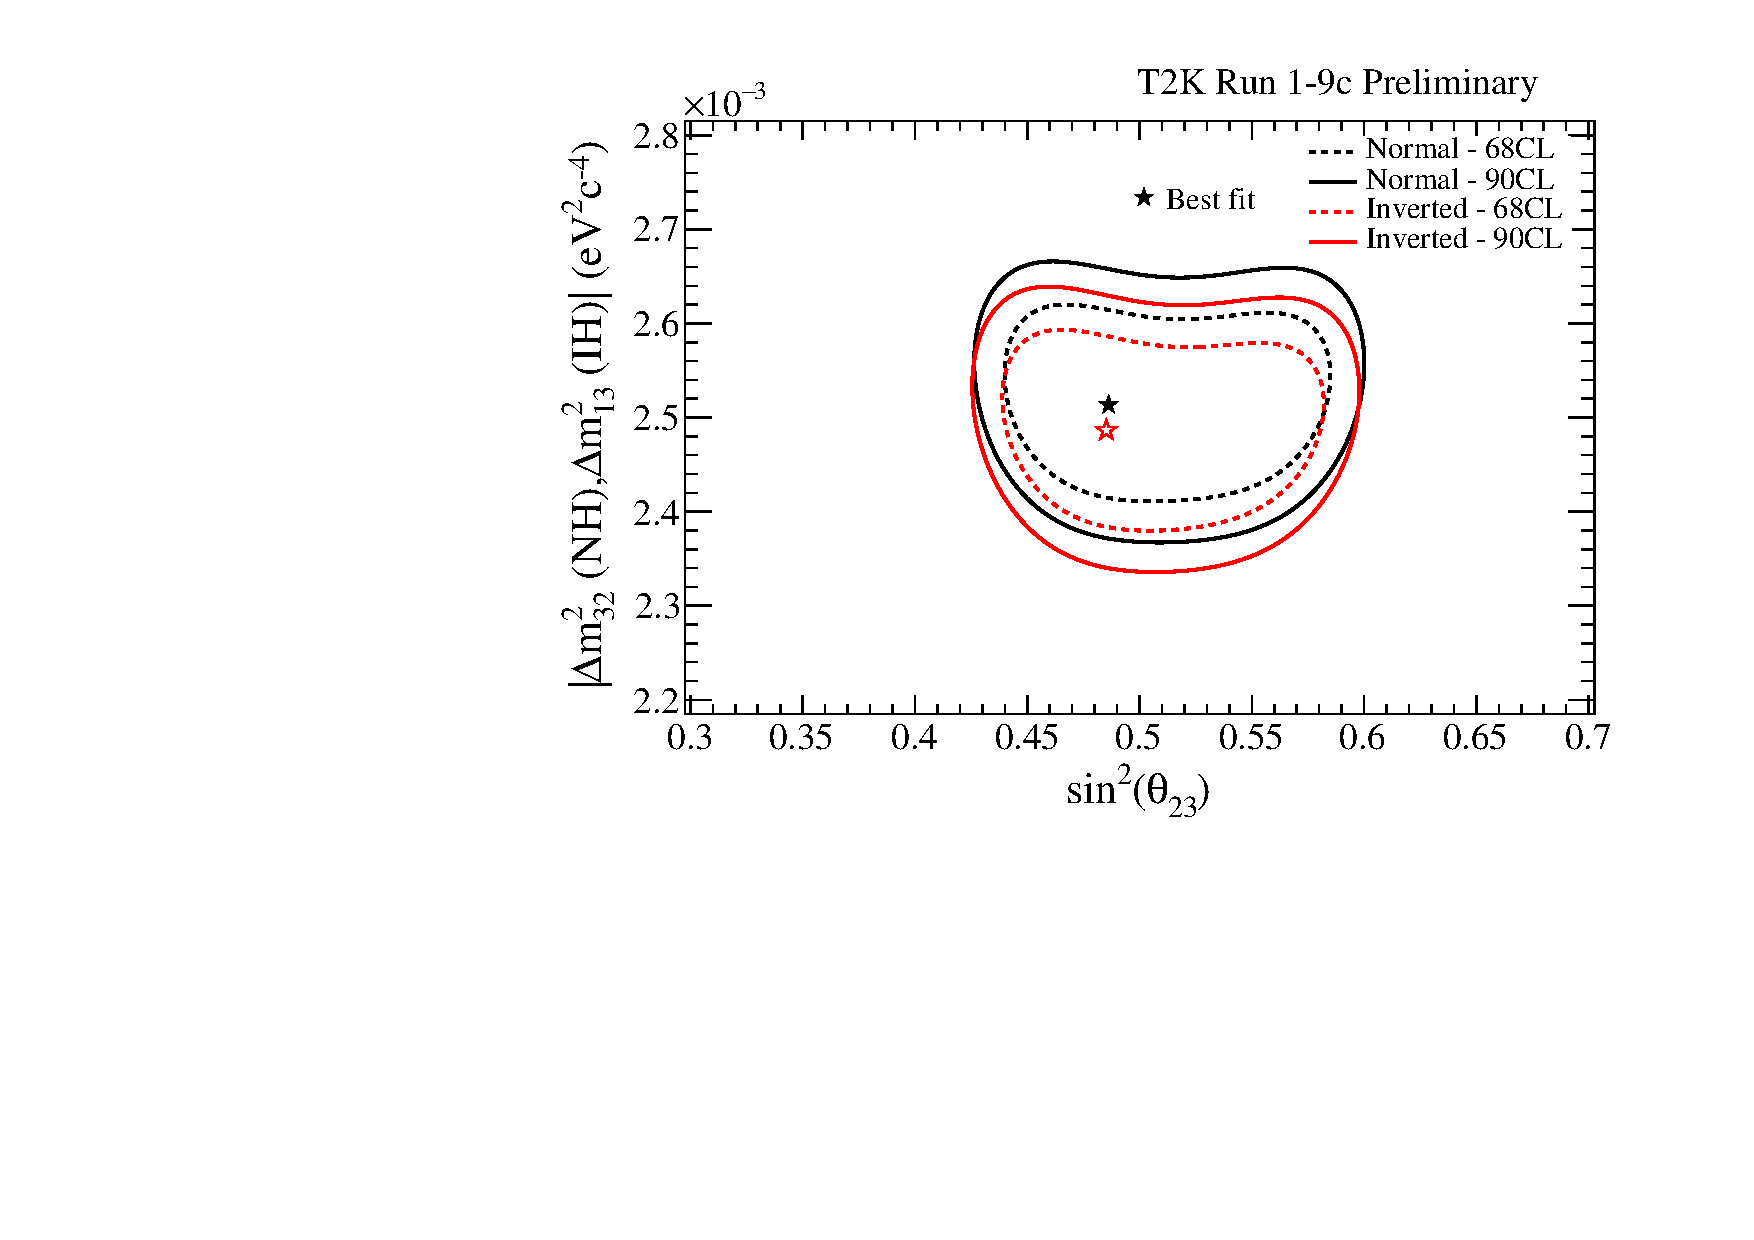
\includegraphics[width=0.9\textwidth]{images/sensitivity/mixing23_dmsq23_AsimovA_t2k_global}
		\caption{Asimov A \disappearance T2K only}
	\end{subfigure}
	\begin{subfigure}[b]{0.49\textwidth}
		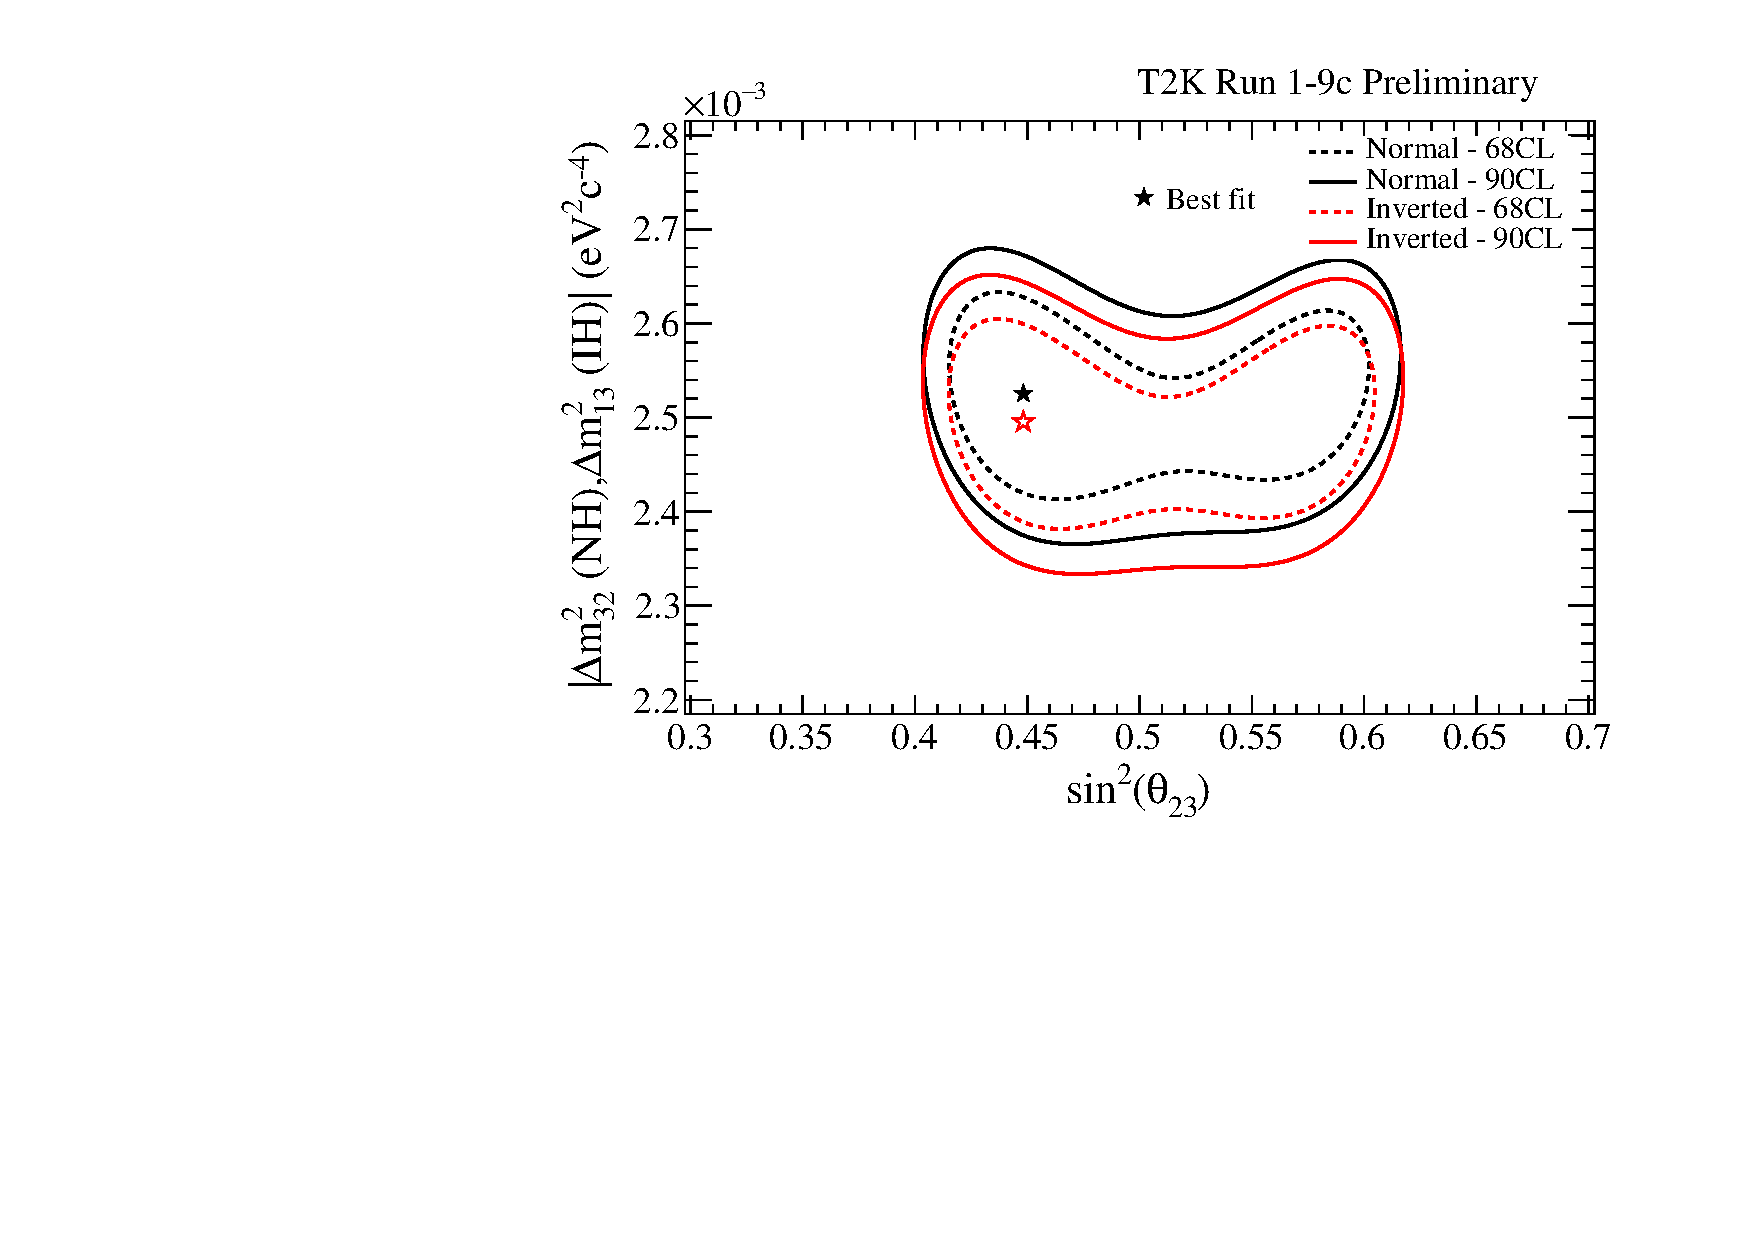
\includegraphics[width=0.9\textwidth]{images/sensitivity/mixing23_dmsq23_AsimovB_reactor_global}
		\caption{Asimov B \disappearance with reactor constraint}
	\end{subfigure}
	\begin{subfigure}[b]{0.49\textwidth}
		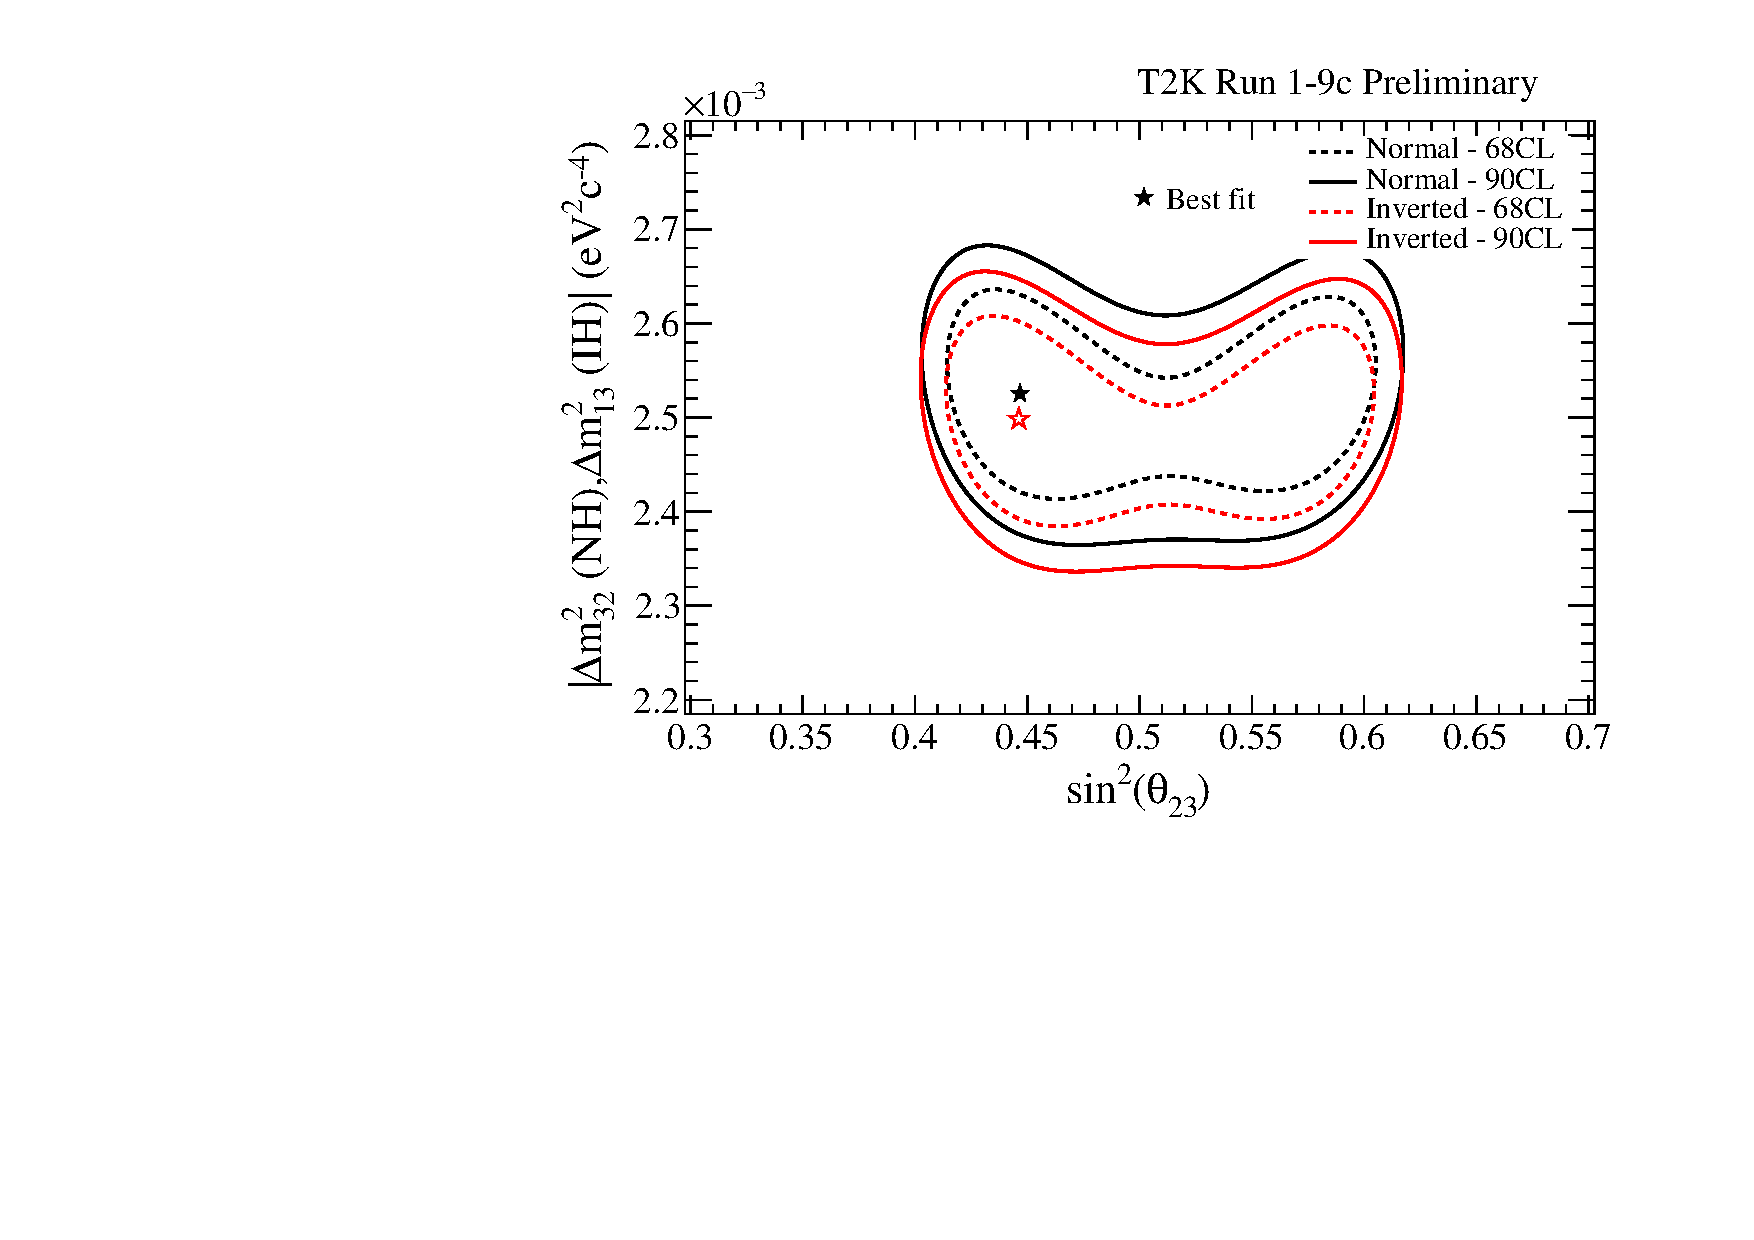
\includegraphics[width=0.9\textwidth]{images/sensitivity/mixing23_dmsq23_AsimovB_t2k_global}
		\caption{Asimov B \disappearance T2K only}
	\end{subfigure}
	\caption {
		Contours at 68\% and 90\% CL for \disappearance with and without reactor constraint for Asimov data sets A and B. Normal and inverted hierarchy contours are independent. All 5 samples were used to produce these fits.
	}
	\label{fig:ssqth23_vs_dmsq23_sensitivity}
\end{figure*}
\clearpage
\subsubsection{Results for \deltacp}

The sensitivity to \deltacp with reactor constraint and T2K only is shown for the Asimov data sets A and B in fig.~\ref{fig:dcp_sensitivity}.

\begin{figure*}[htb]
	\center
	\begin{subfigure}[b]{0.49\textwidth}
		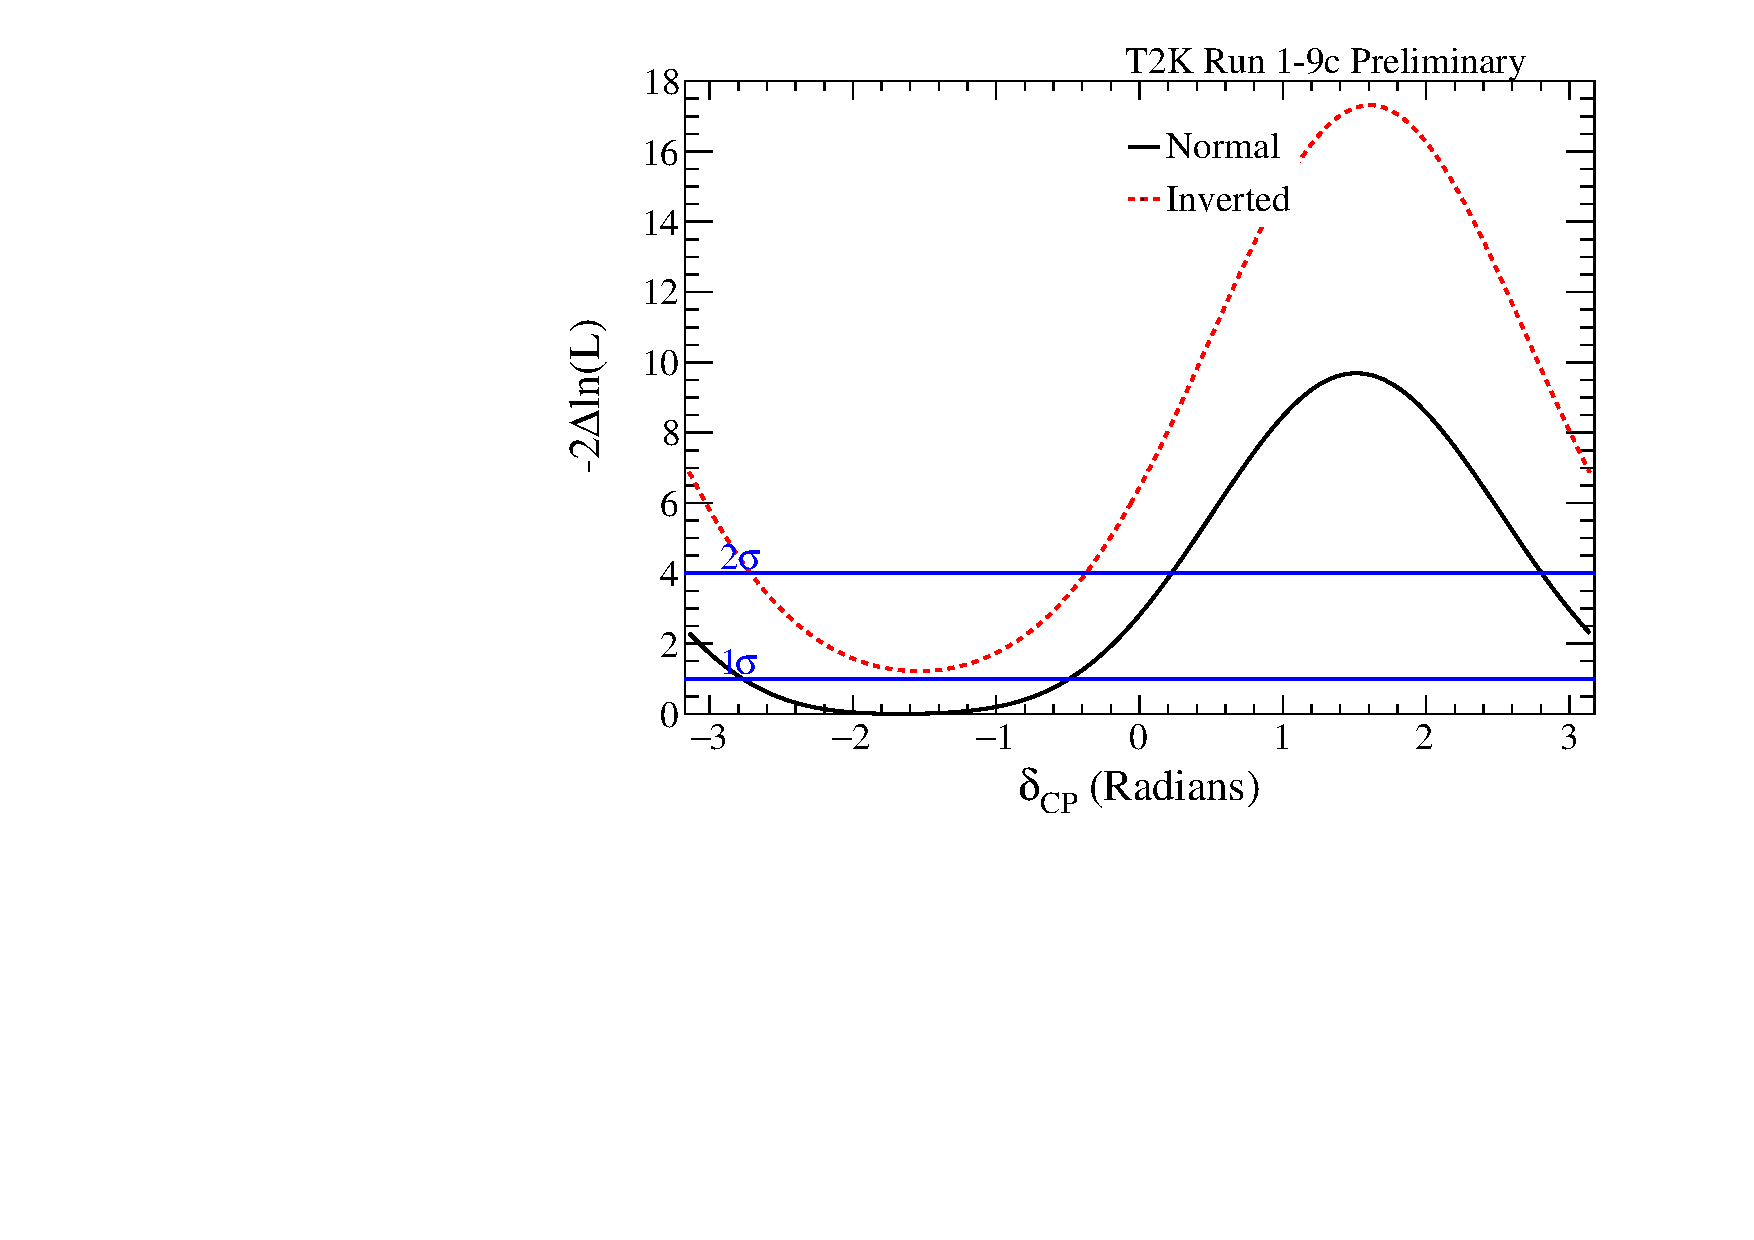
\includegraphics[width=0.9\textwidth]{images/sensitivity/deltacp_AsimovA_reactor_global}
		\caption{Asimov A \deltacp with reactor constraint}
	\end{subfigure}
	\begin{subfigure}[b]{0.49\textwidth}
		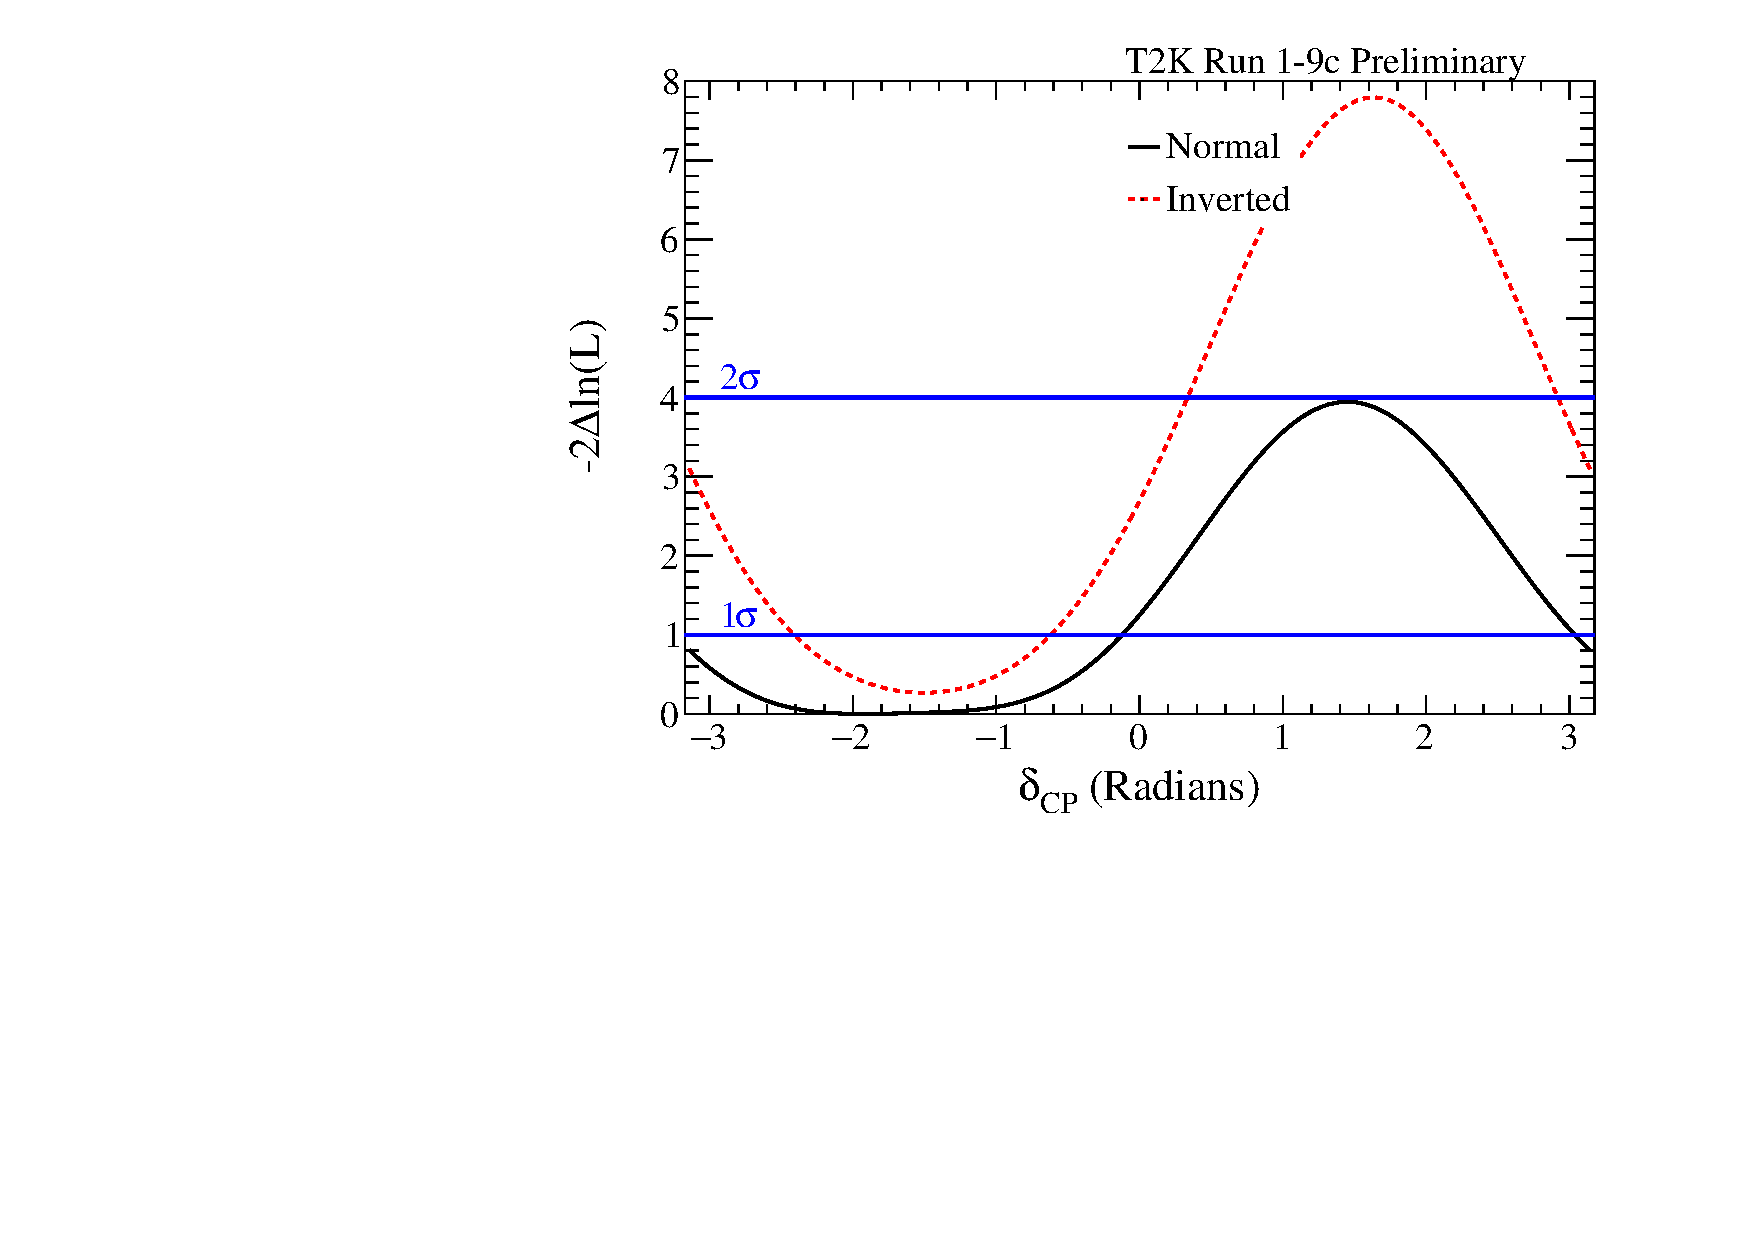
\includegraphics[width=0.9\textwidth]{images/sensitivity/deltacp_AsimovA_t2k_global}
		\caption{Asimov A \deltacp T2K only}
	\end{subfigure}
	\begin{subfigure}[b]{0.49\textwidth}
		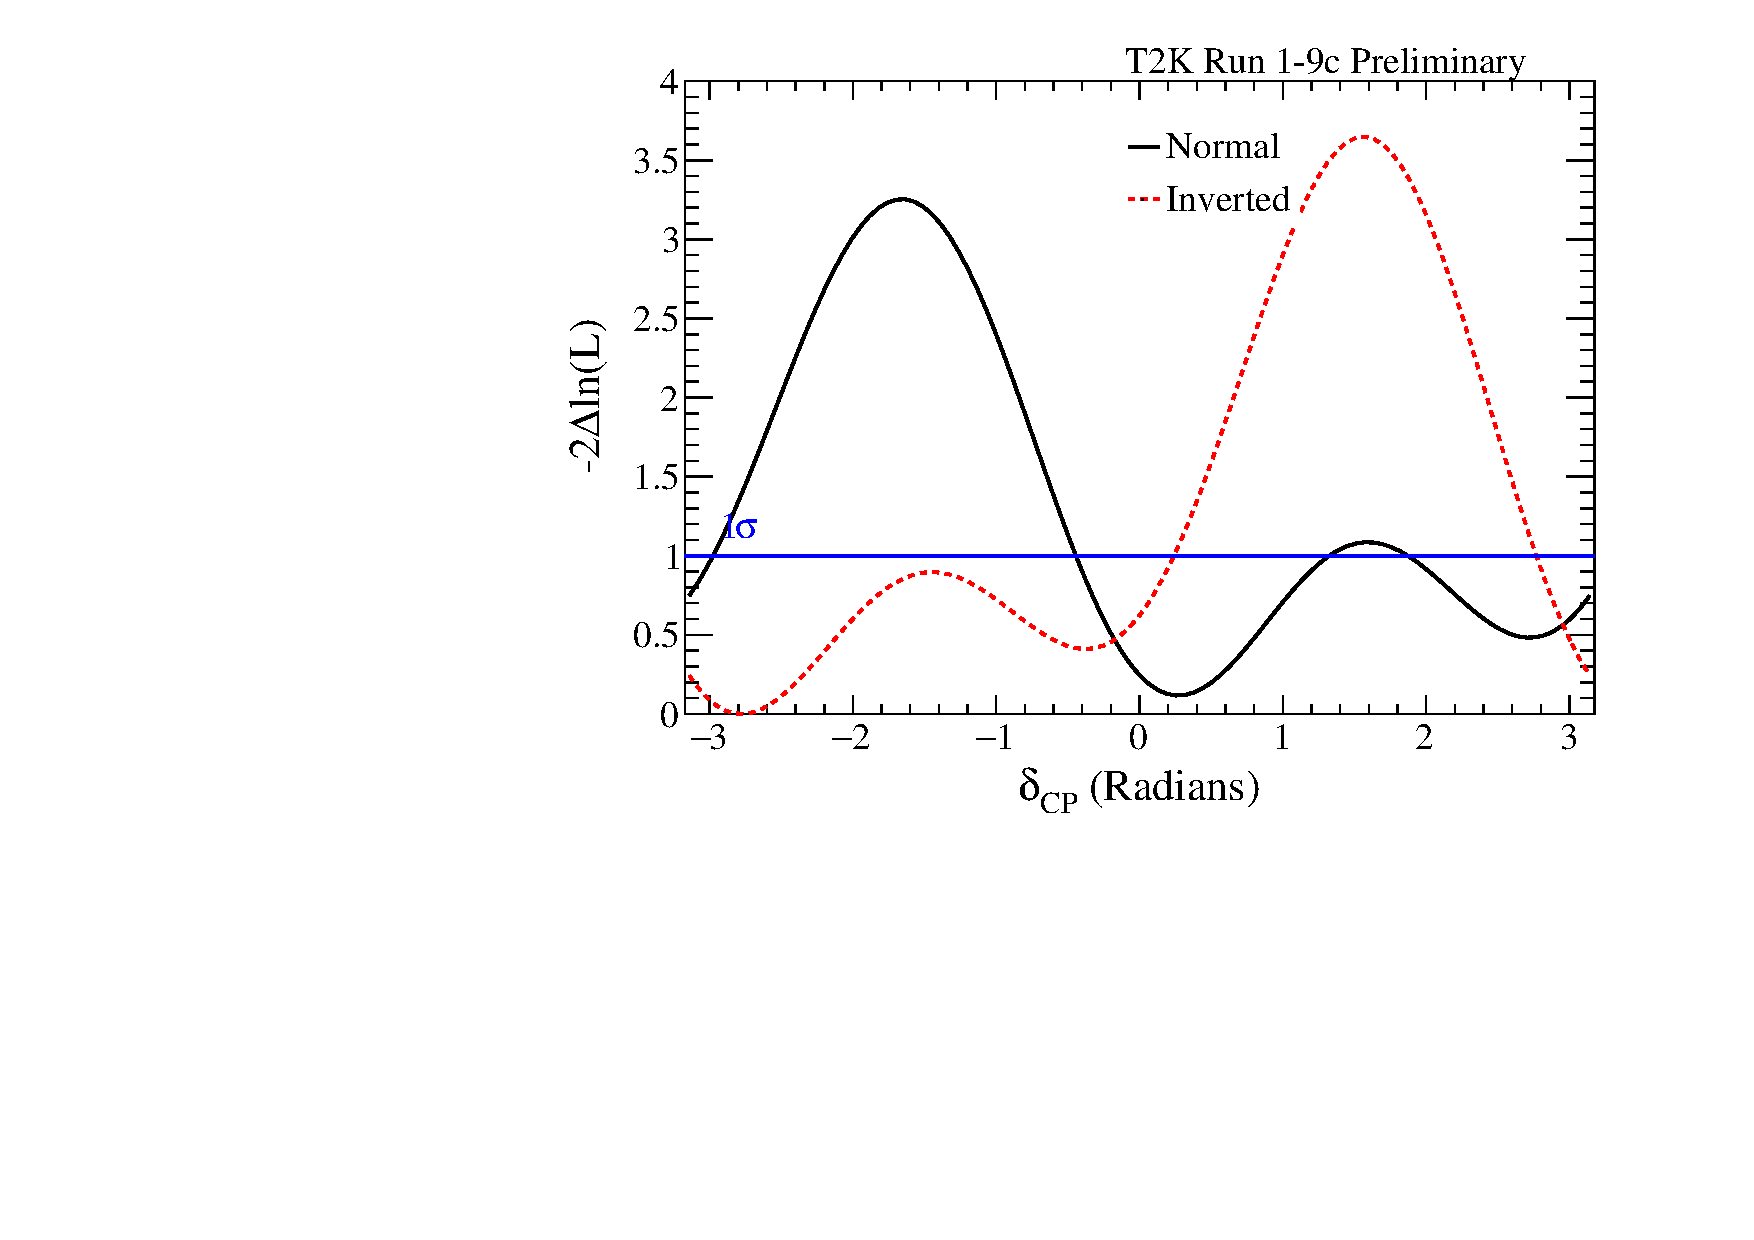
\includegraphics[width=0.9\textwidth]{images/sensitivity/deltacp_AsimovB_reactor_global}
		\caption{Asimov B \deltacp with reactor constraint}
	\end{subfigure}
	\begin{subfigure}[b]{0.49\textwidth}
		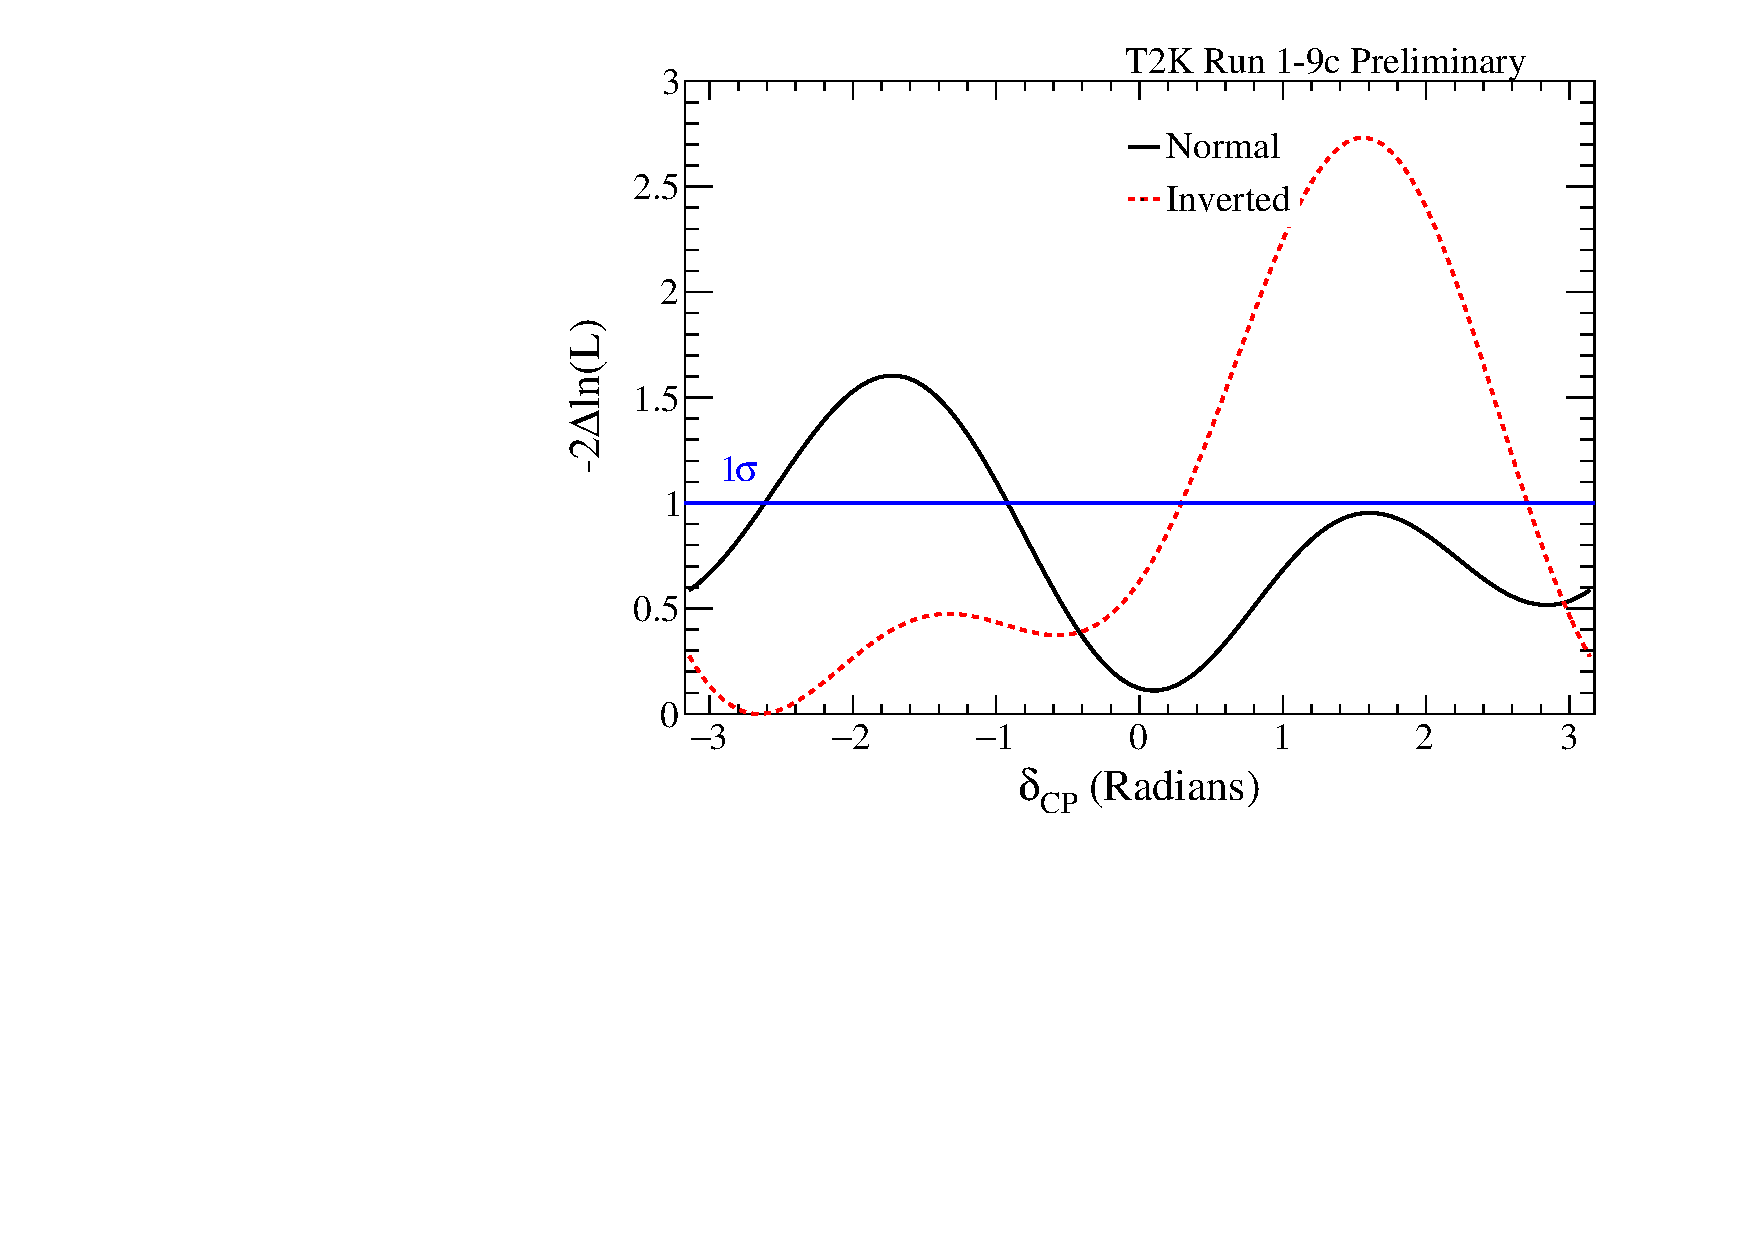
\includegraphics[width=0.9\textwidth]{images/sensitivity/deltacp_AsimovB_t2k_global}
		\caption{Asimov B \deltacp T2K only}
	\end{subfigure}
	\caption {
		The expected $\Delta\chi^2$ distribution as a function of \deltacp with and without reactor constraint for Asimov data sets A and B. The mass hierarchy is minimized, with normal and inverted hierarchy $\Delta\chi^2$ distributions shifted to the same global best-fit $\chi^2$ value, which is taken to be the minimum between normal and inverted hierarchy. All 5 samples were used to produce these fits.
	}
	\label{fig:dcp_sensitivity}
\end{figure*}
\clearpage
\subsubsection{Results for \ssqthonethree}

The sensitivity to \ssqthonethree (without reactor constraint) is shown for the Asimov data sets A and B in fig.~\ref{fig:th13_sensitivity}.

\begin{figure*}[htb]
	\center
	\begin{subfigure}[b]{0.49\textwidth}
		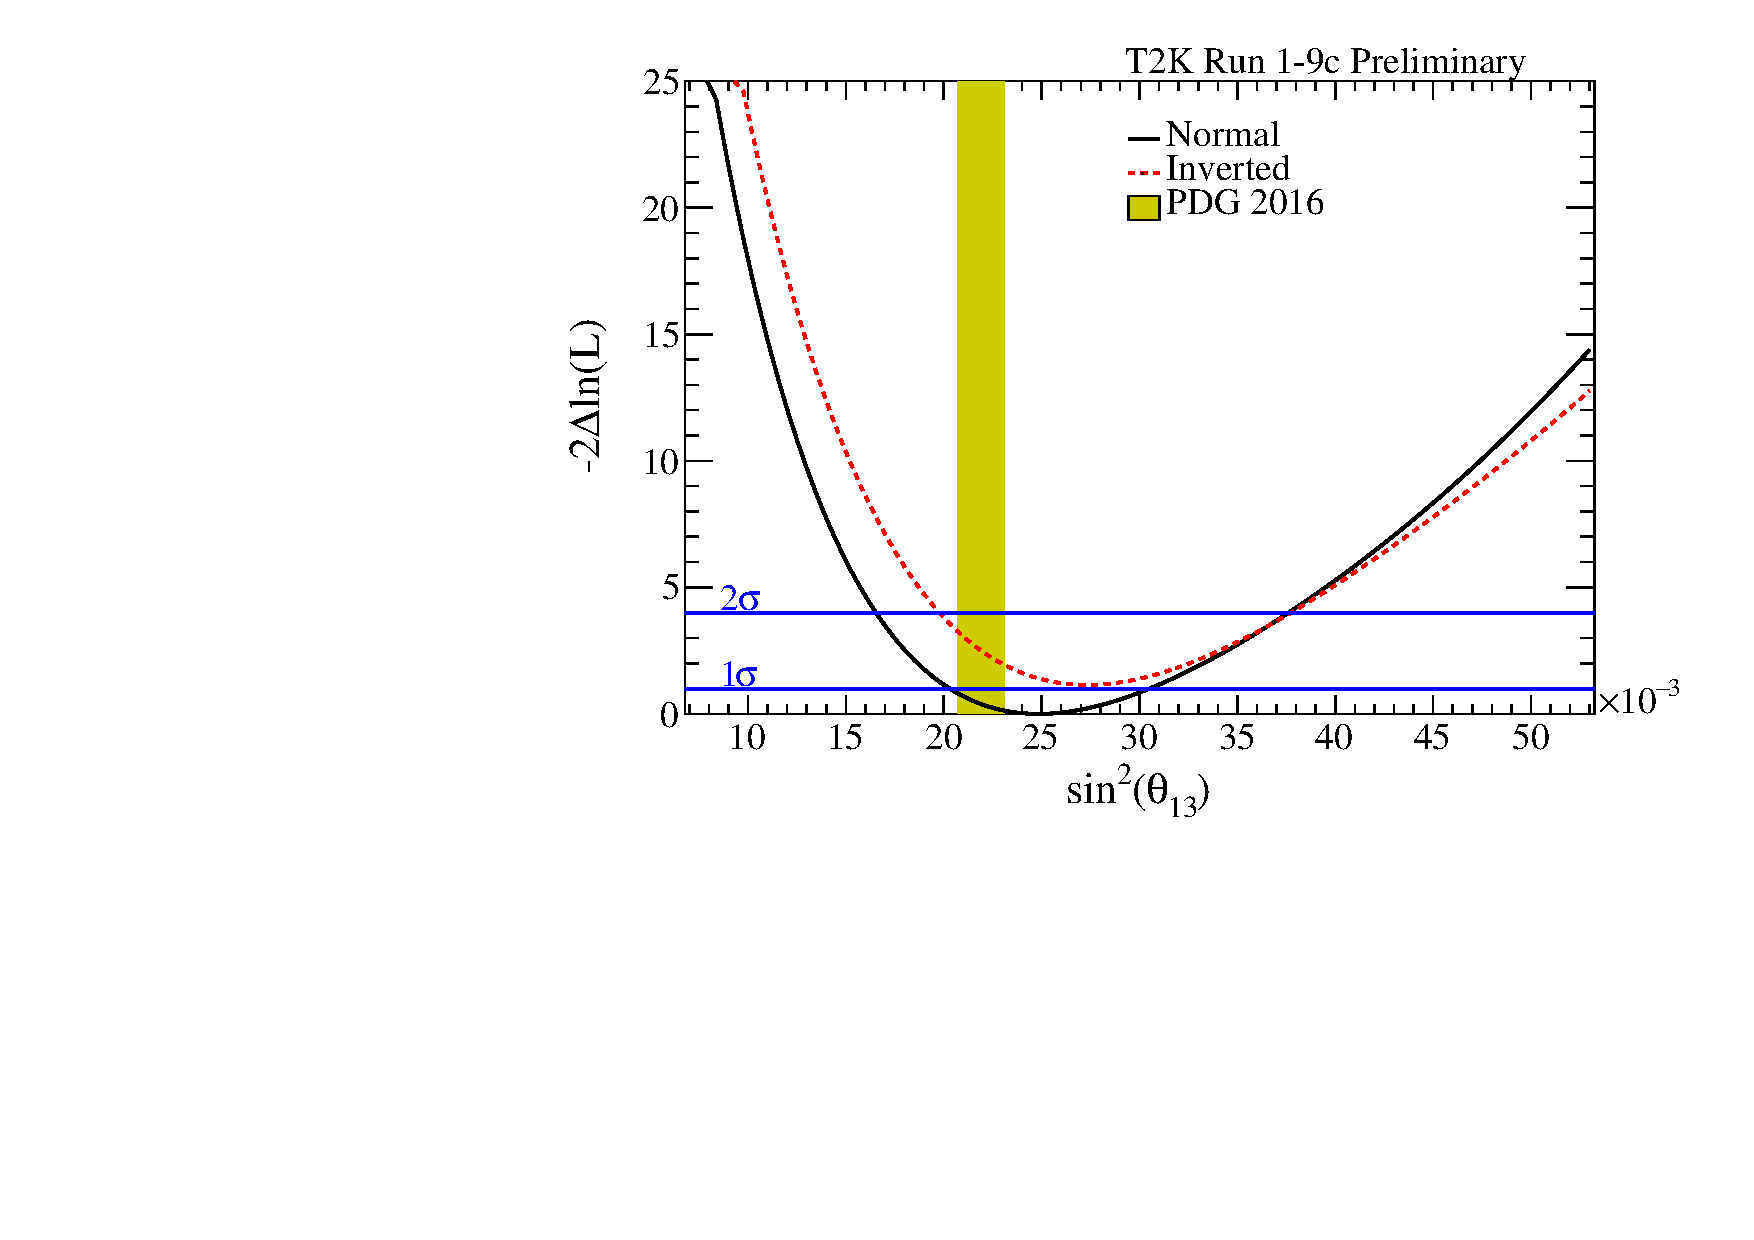
\includegraphics[width=0.9\textwidth]{images/sensitivity/mixing13_AsimovA_t2k_global}
		\caption{Asimov A \ssqthonethree T2K only}
	\end{subfigure}
	\begin{subfigure}[b]{0.49\textwidth}
		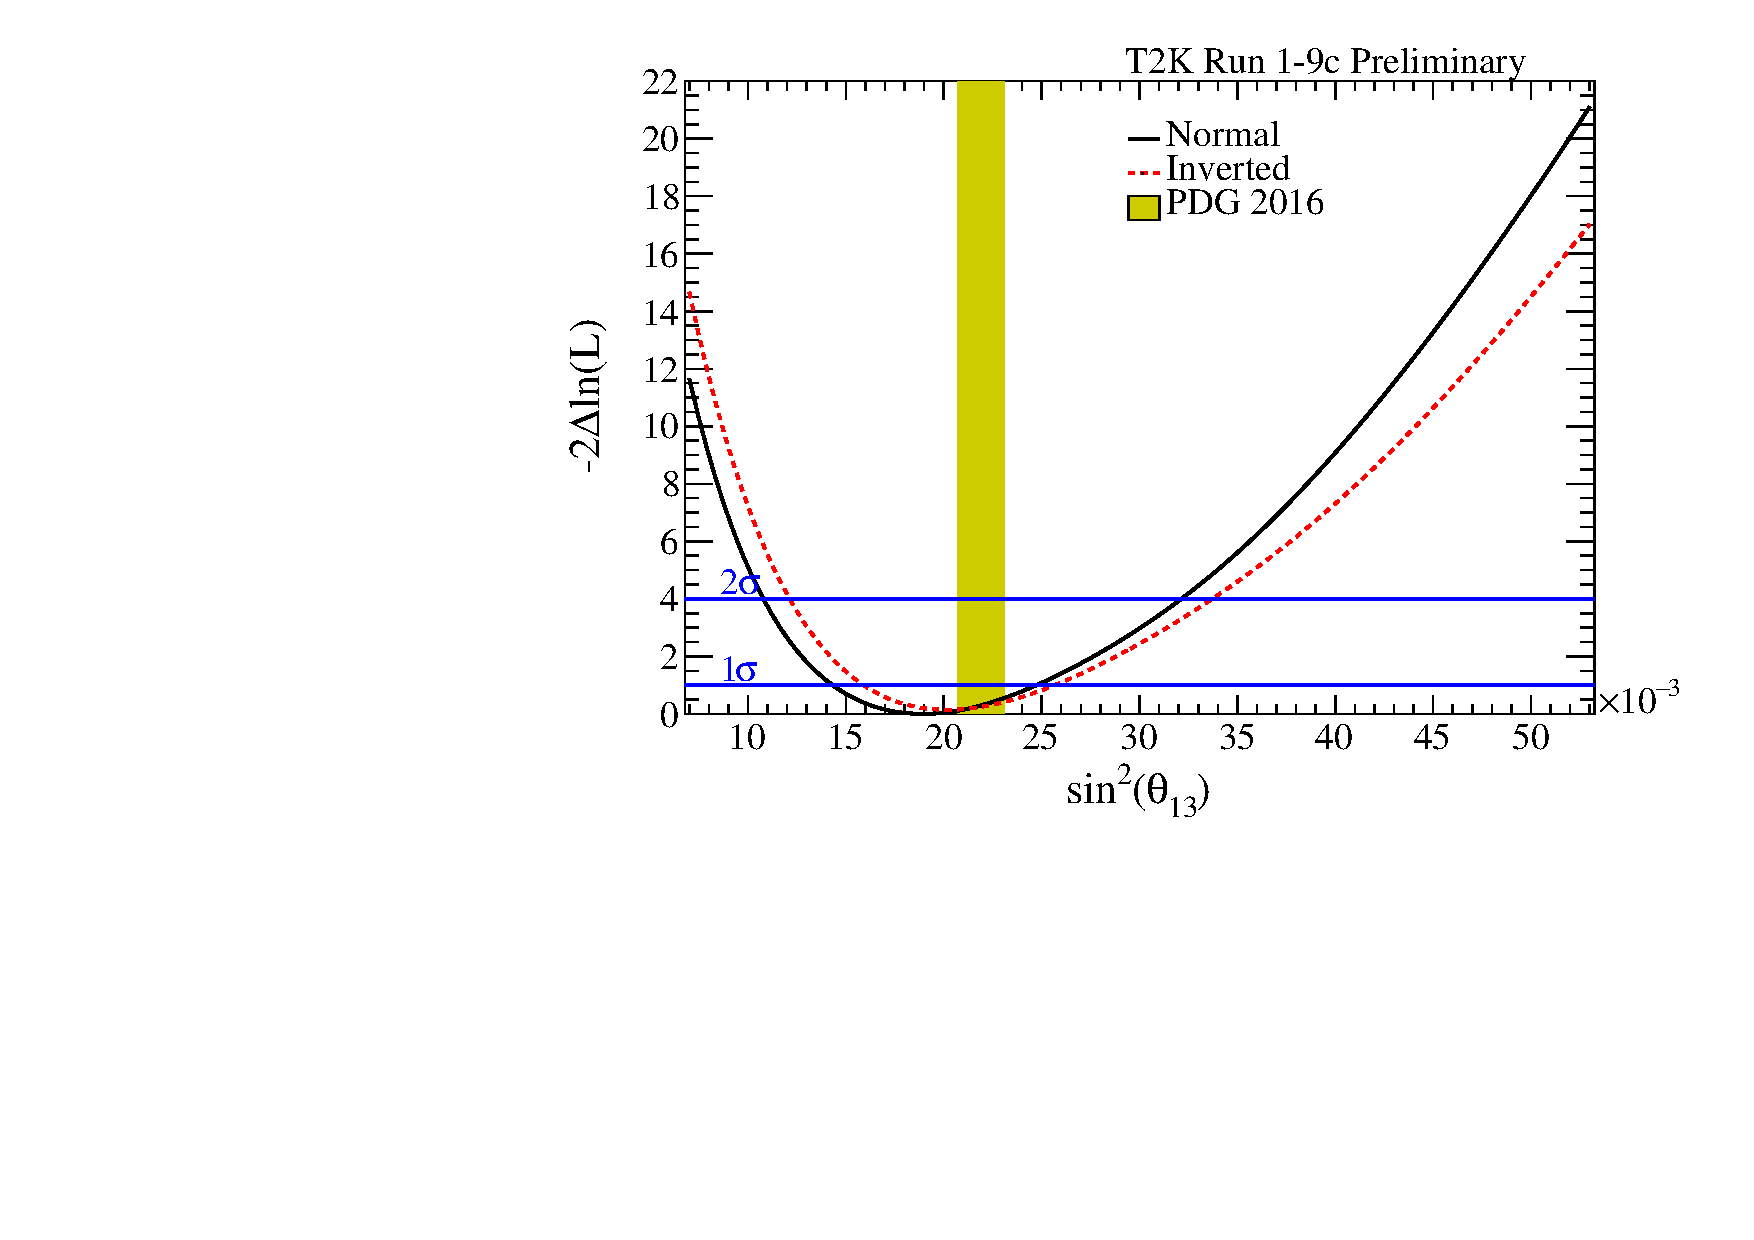
\includegraphics[width=0.9\textwidth]{images/sensitivity/mixing13_AsimovB_t2k_global}
		\caption{Asimov B \ssqthonethree T2K only}
	\end{subfigure}
	\caption {
		The expected $\Delta\chi^2$ distribution as a function of \ssqthonethree without reactor constraint for Asimov data sets A and B. The mass hierarchy is minimized, with normal and inverted hierarchy $\Delta\chi^2$ distributions shifted to the same global best-fit $\chi^2$ value, which is taken to be the minimum between normal and inverted hierarchy. All 5 samples were used to produce these fits.
	}
	\label{fig:th13_sensitivity}
\end{figure*}
\clearpage
\subsubsection{Results for \ssqthtwothree}

The sensitivity to \ssqthtwothree with reactor constraint and T2K only is shown for the Asimov data sets A and B in fig.~\ref{fig:th23_sensitivity}.

\begin{figure*}[htb]
	\center
	\begin{subfigure}[b]{0.49\textwidth}
		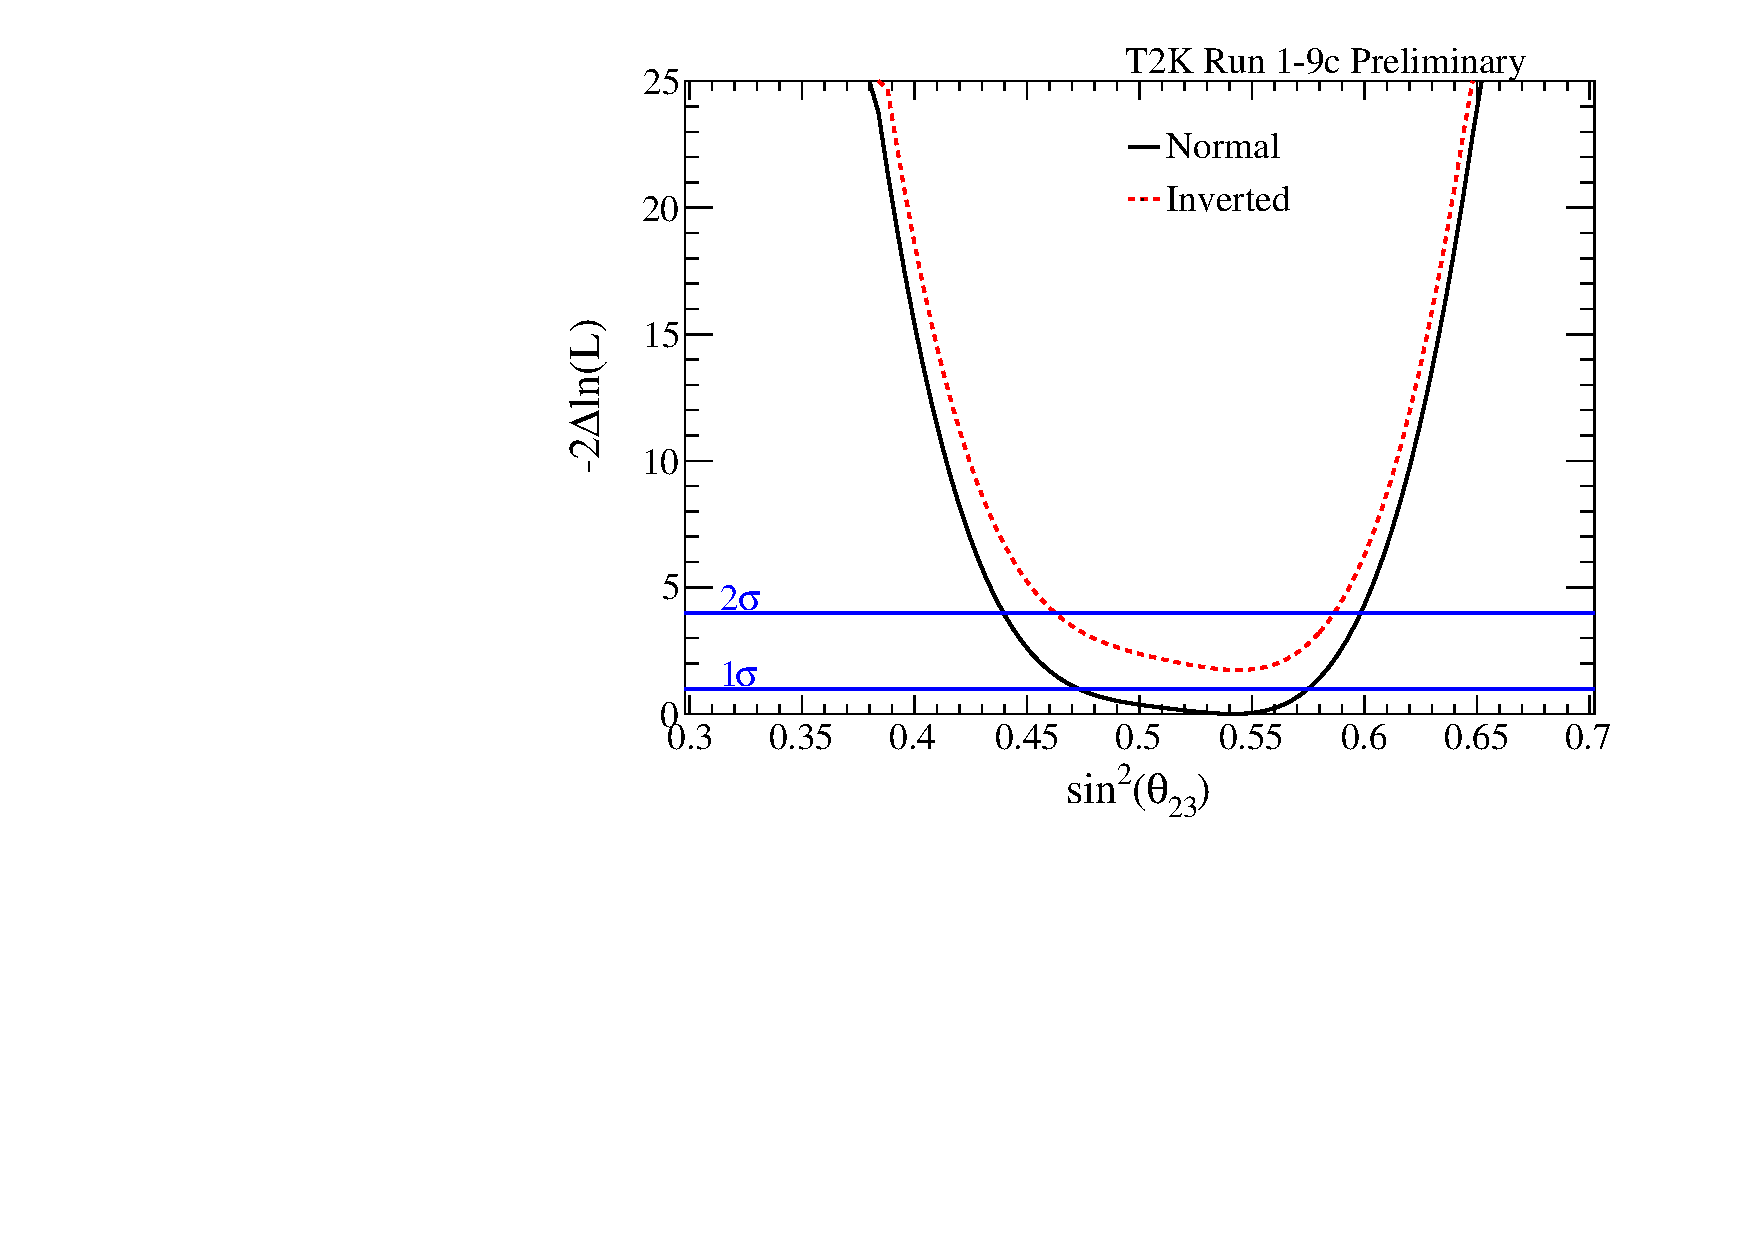
\includegraphics[width=0.9\textwidth]{images/sensitivity/mixing23_AsimovA_reactor_global}
		\caption{Asimov A \ssqthtwothree with reactor constraint}
	\end{subfigure}
	\begin{subfigure}[b]{0.49\textwidth}
		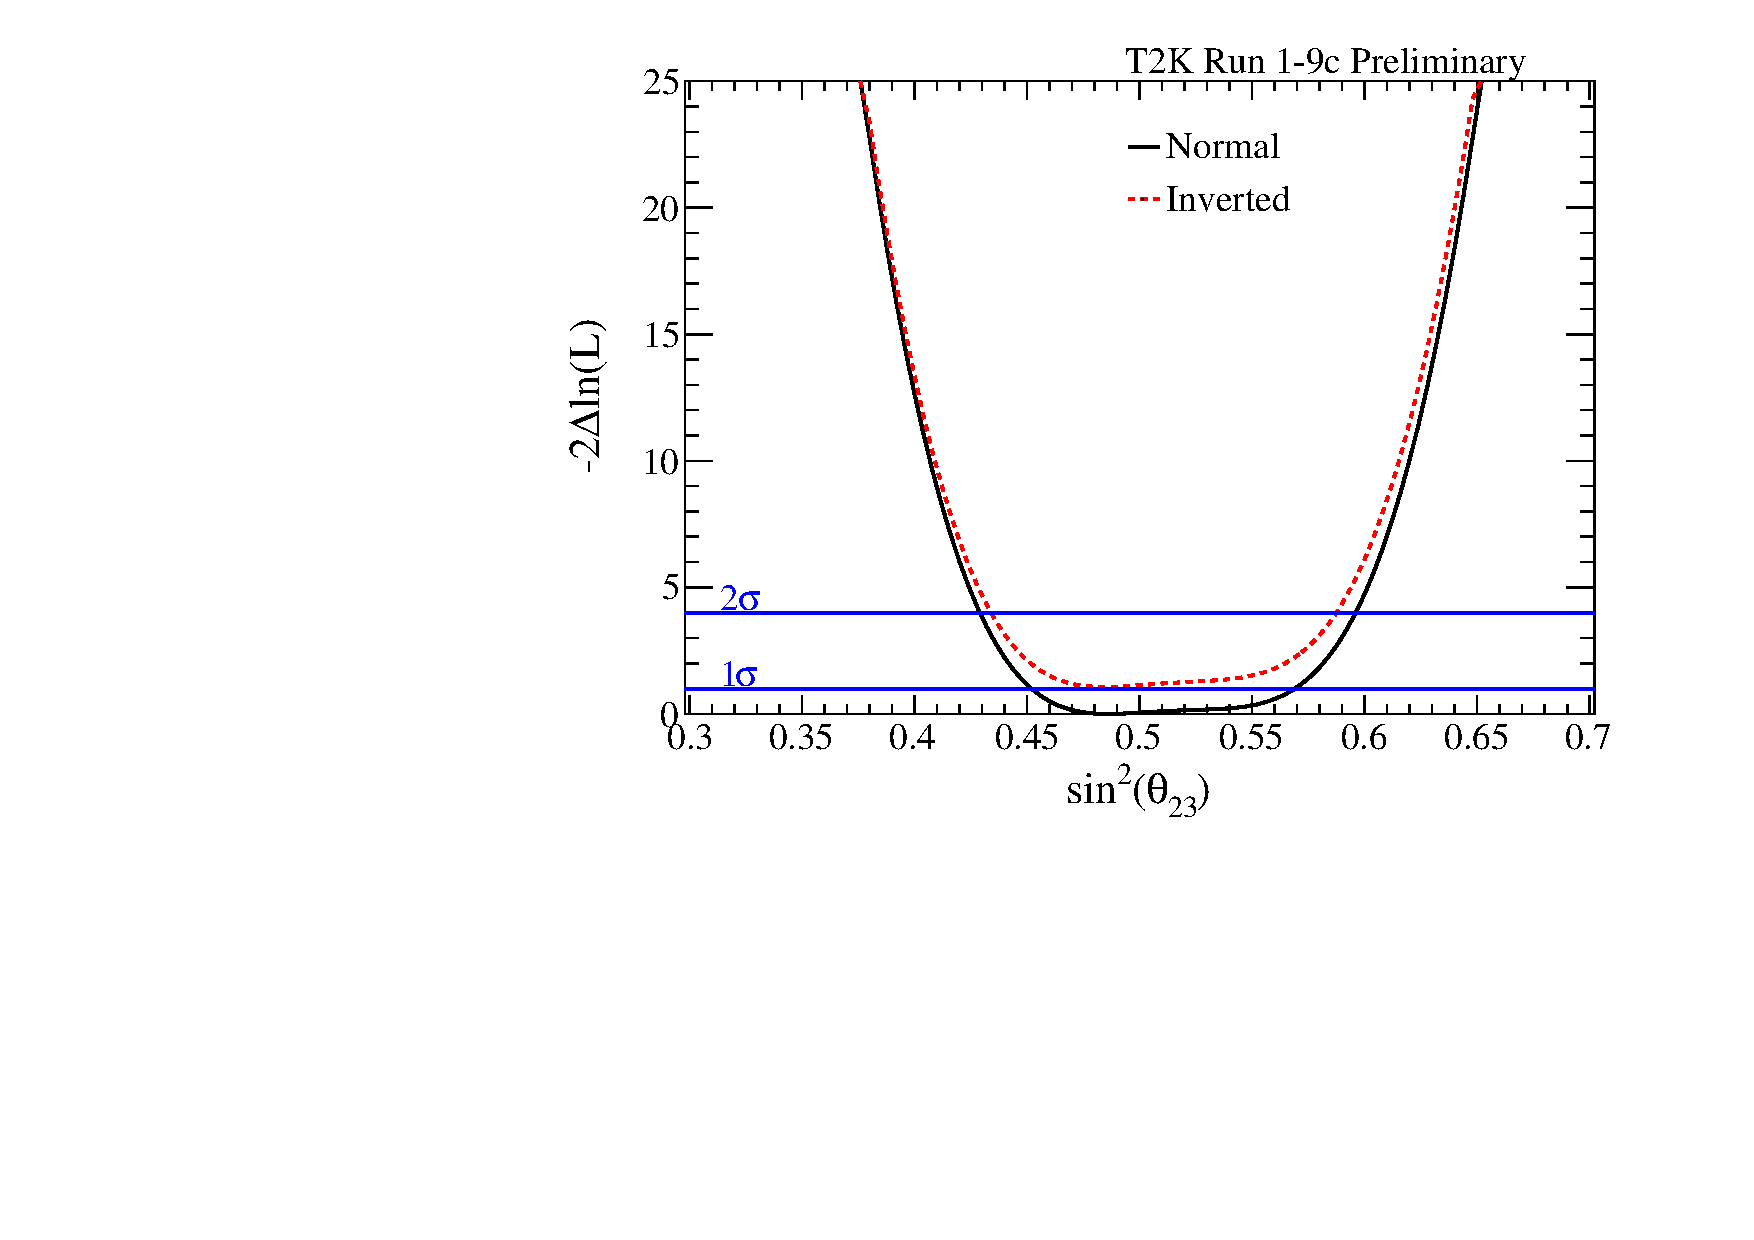
\includegraphics[width=0.9\textwidth]{images/sensitivity/mixing23_AsimovA_t2k_global}
		\caption{Asimov A \ssqthtwothree T2K only}
	\end{subfigure}
	\begin{subfigure}[b]{0.49\textwidth}
		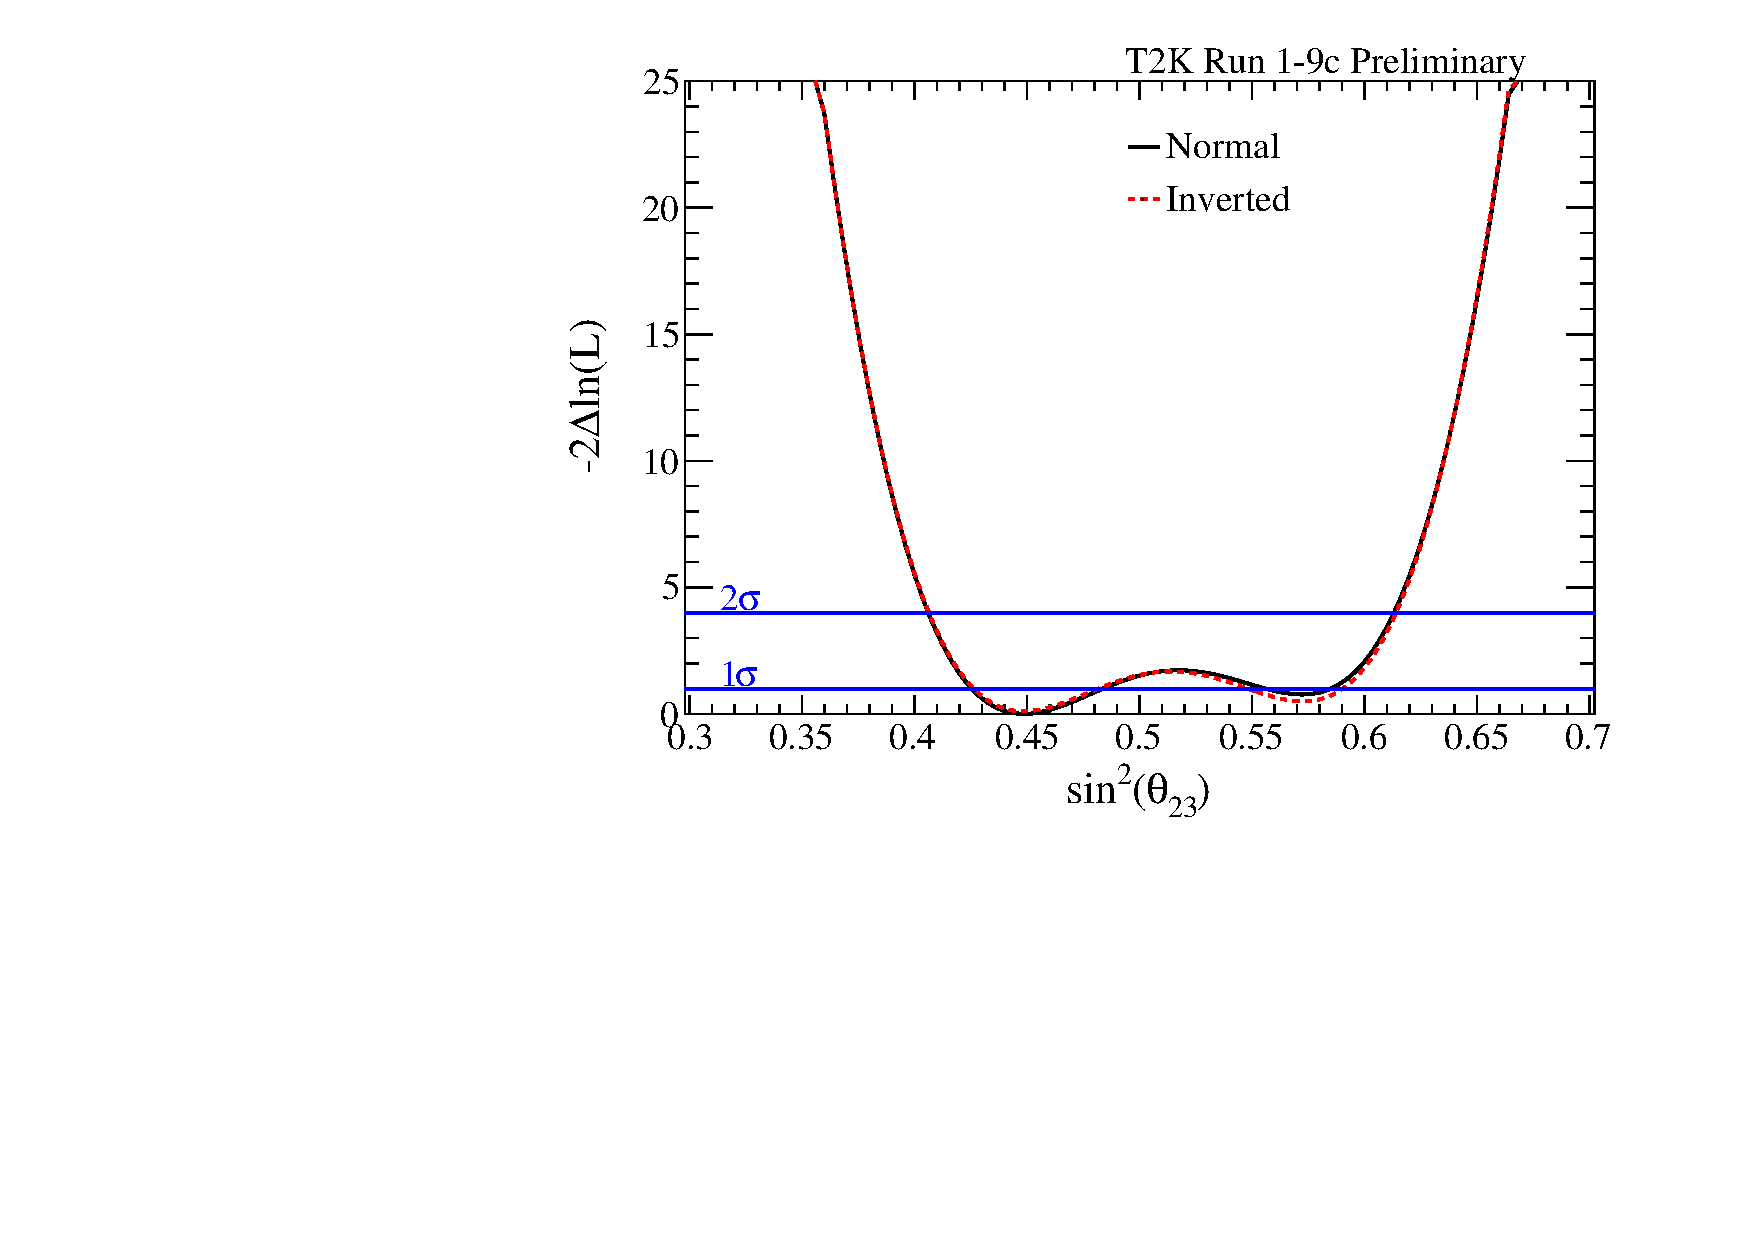
\includegraphics[width=0.9\textwidth]{images/sensitivity/mixing23_AsimovB_reactor_global}
		\caption{Asimov B \ssqthtwothree with reactor constraint}
	\end{subfigure}
	\begin{subfigure}[b]{0.49\textwidth}
		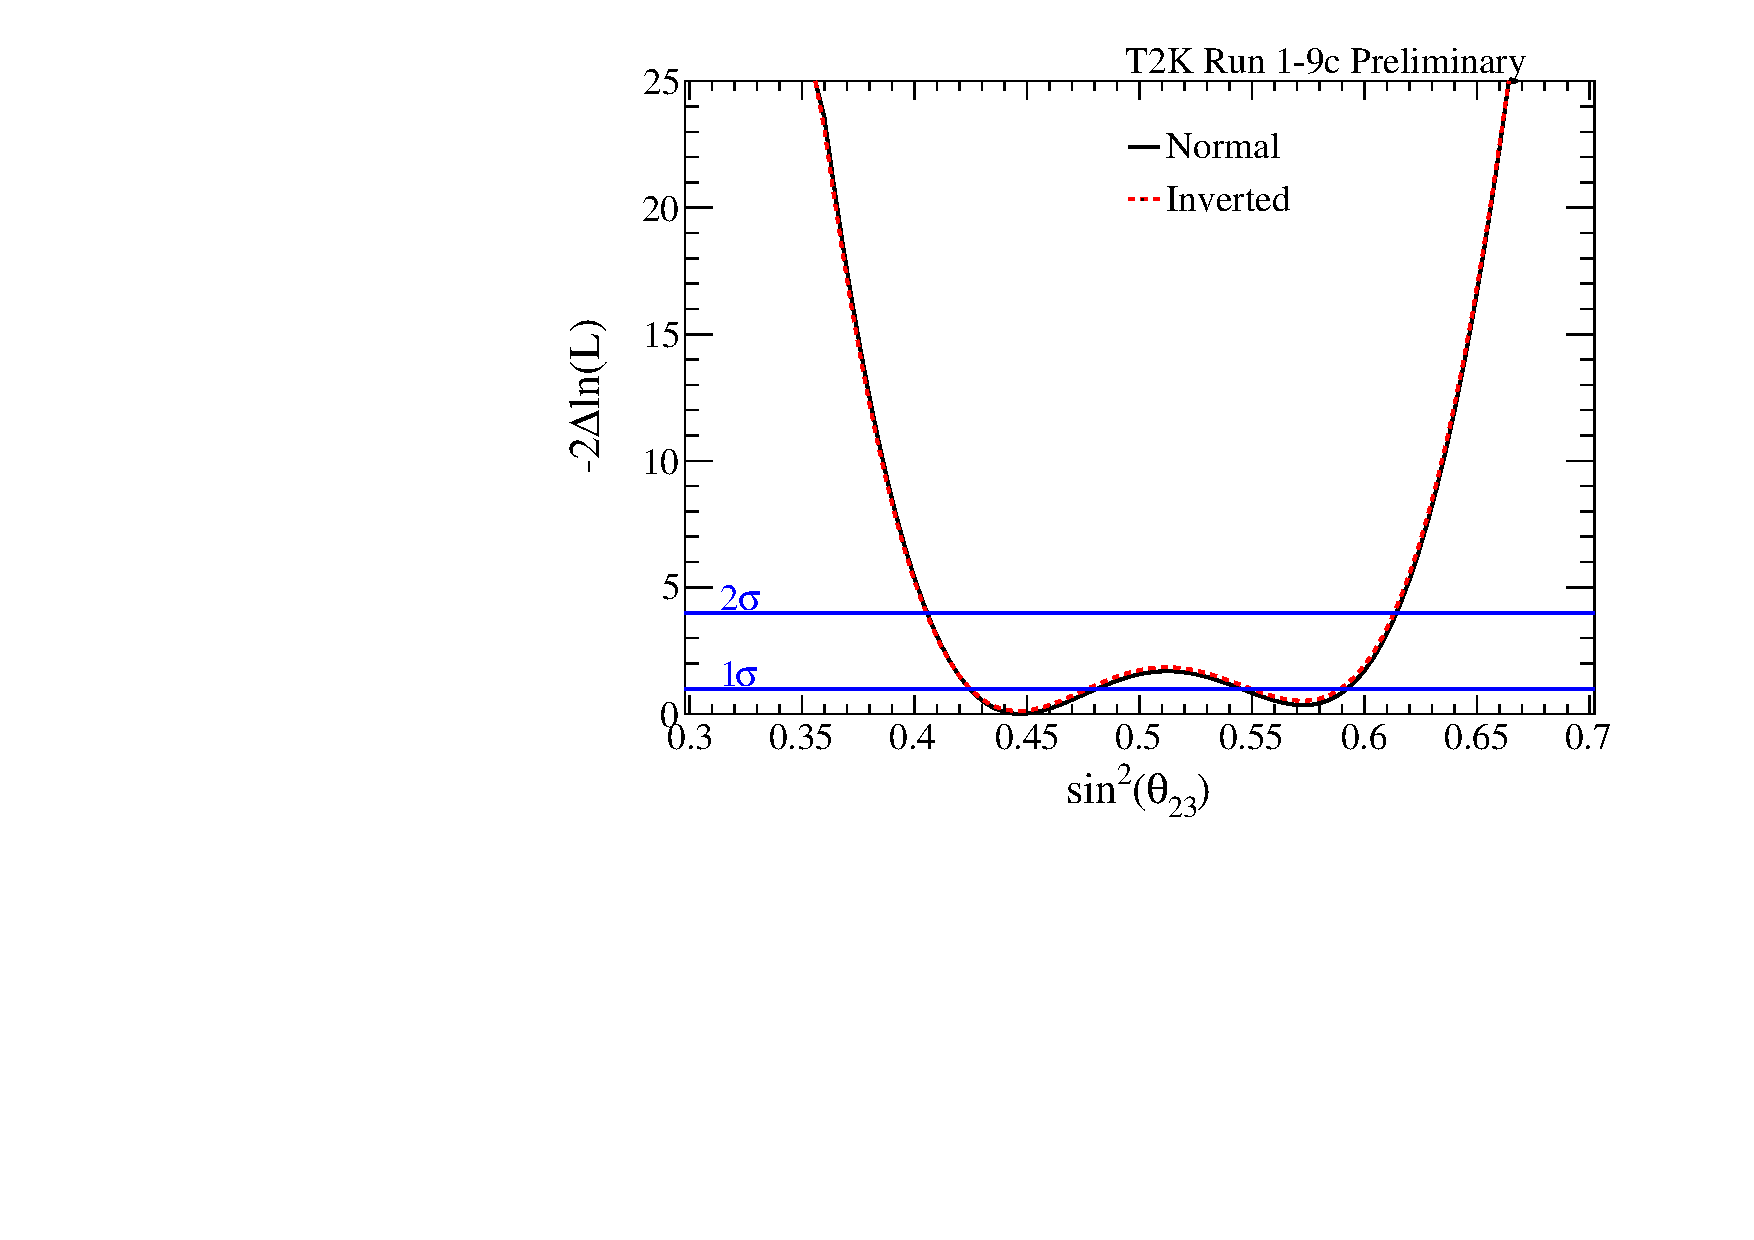
\includegraphics[width=0.9\textwidth]{images/sensitivity/mixing23_AsimovB_t2k_global}
		\caption{Asimov B \ssqthtwothree T2K only}
	\end{subfigure}
	\caption {
		The expected $\Delta\chi^2$ distribution as a function of \ssqthtwothree with and without reactor constraint for Asimov data sets A and B. The mass hierarchy is minimized, with normal and inverted hierarchy $\Delta\chi^2$ distributions shifted to the same global best-fit $\chi^2$ value, which is taken to be the minimum between normal and inverted hierarchy. All 5 samples were used to produce these fits.
	}
	\label{fig:th23_sensitivity}
\end{figure*}
\clearpage
\subsubsection{Results for \dmsq}

The sensitivity to \dmsq with reactor constraint and T2K only is shown for the Asimov data sets A and B in fig.~\ref{fig:dmsq23_sensitivity}.

\begin{figure*}[htb]
	\center
	\begin{subfigure}[b]{0.49\textwidth}
		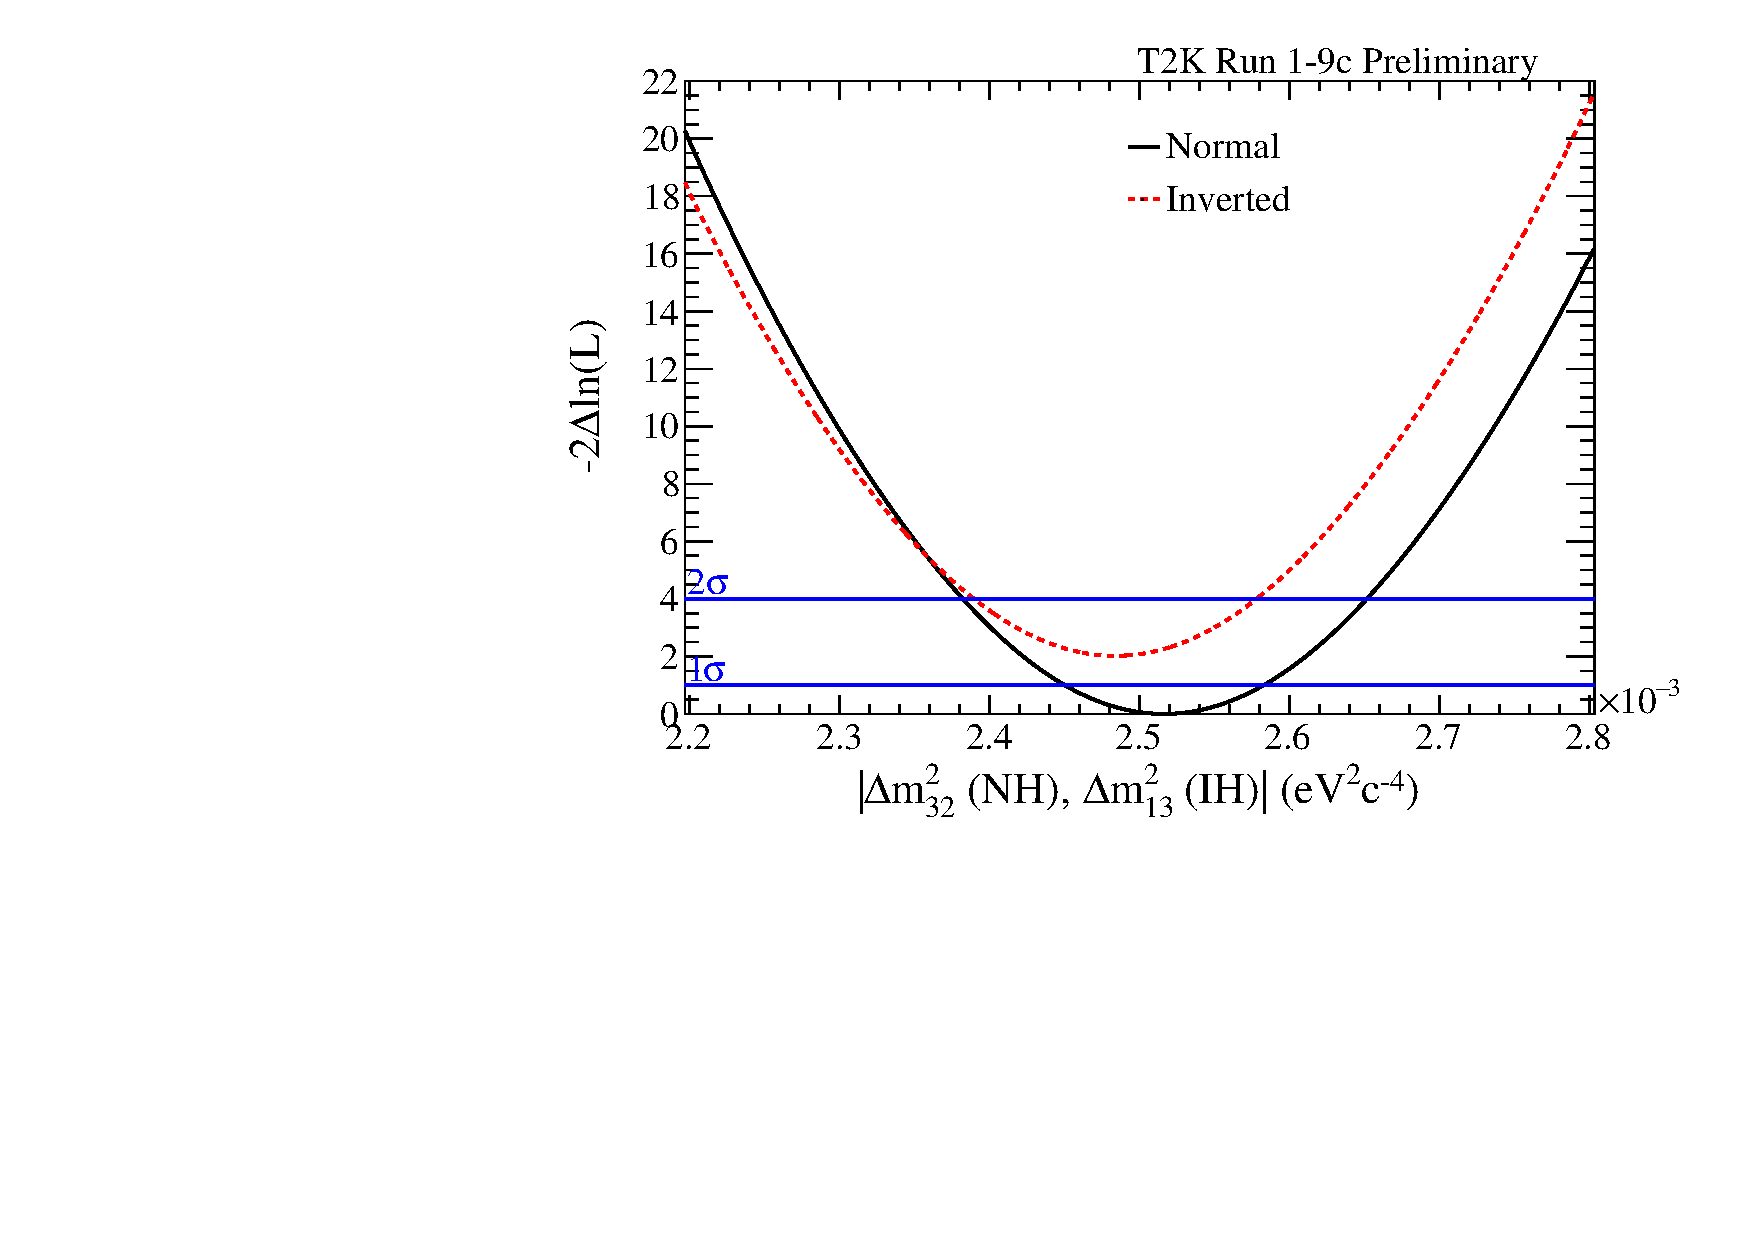
\includegraphics[width=0.9\textwidth]{images/sensitivity/dmsq23_AsimovA_reactor_global}
		\caption{Asimov A \dmsq with reactor constraint}
	\end{subfigure}
	\begin{subfigure}[b]{0.49\textwidth}
		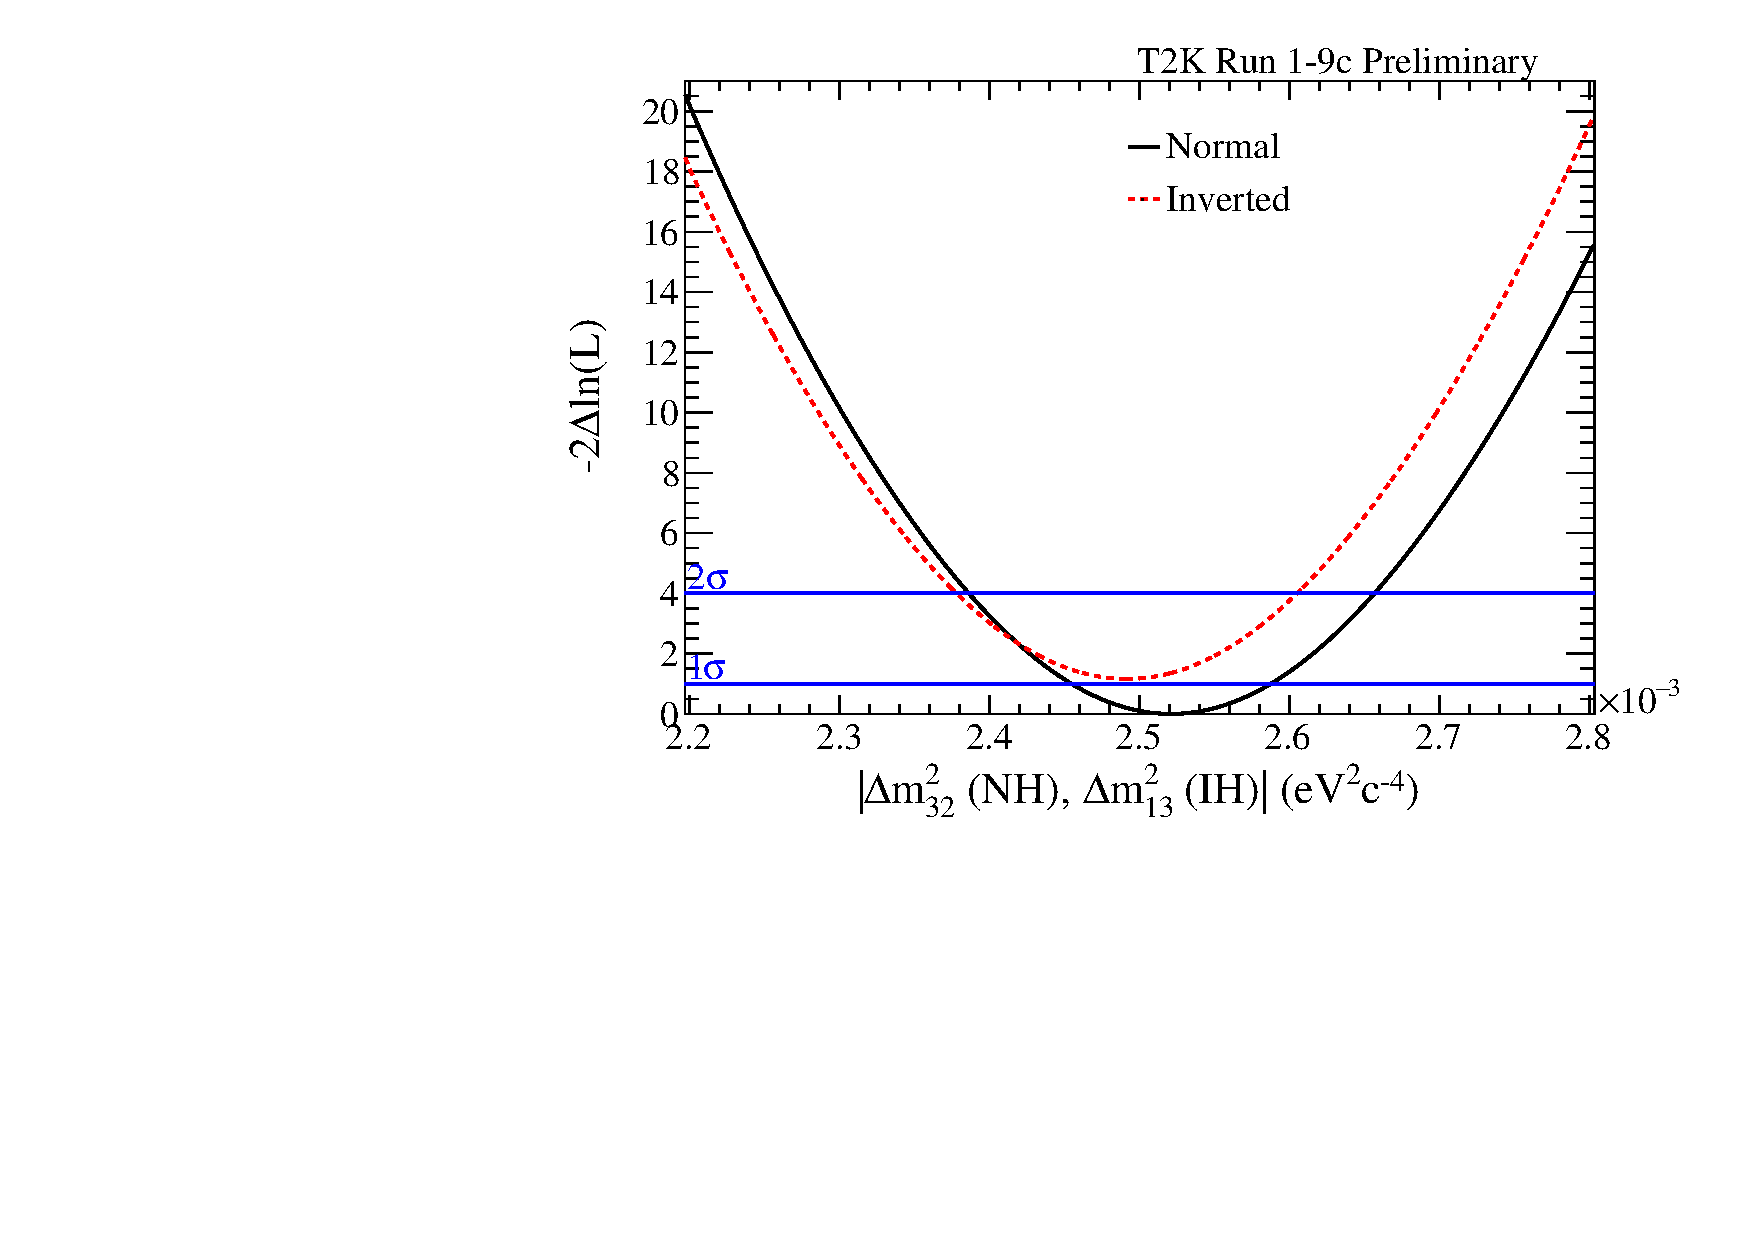
\includegraphics[width=0.9\textwidth]{images/sensitivity/dmsq23_AsimovA_t2k_global}
		\caption{Asimov A \dmsq T2K only}
	\end{subfigure}
	\begin{subfigure}[b]{0.49\textwidth}
		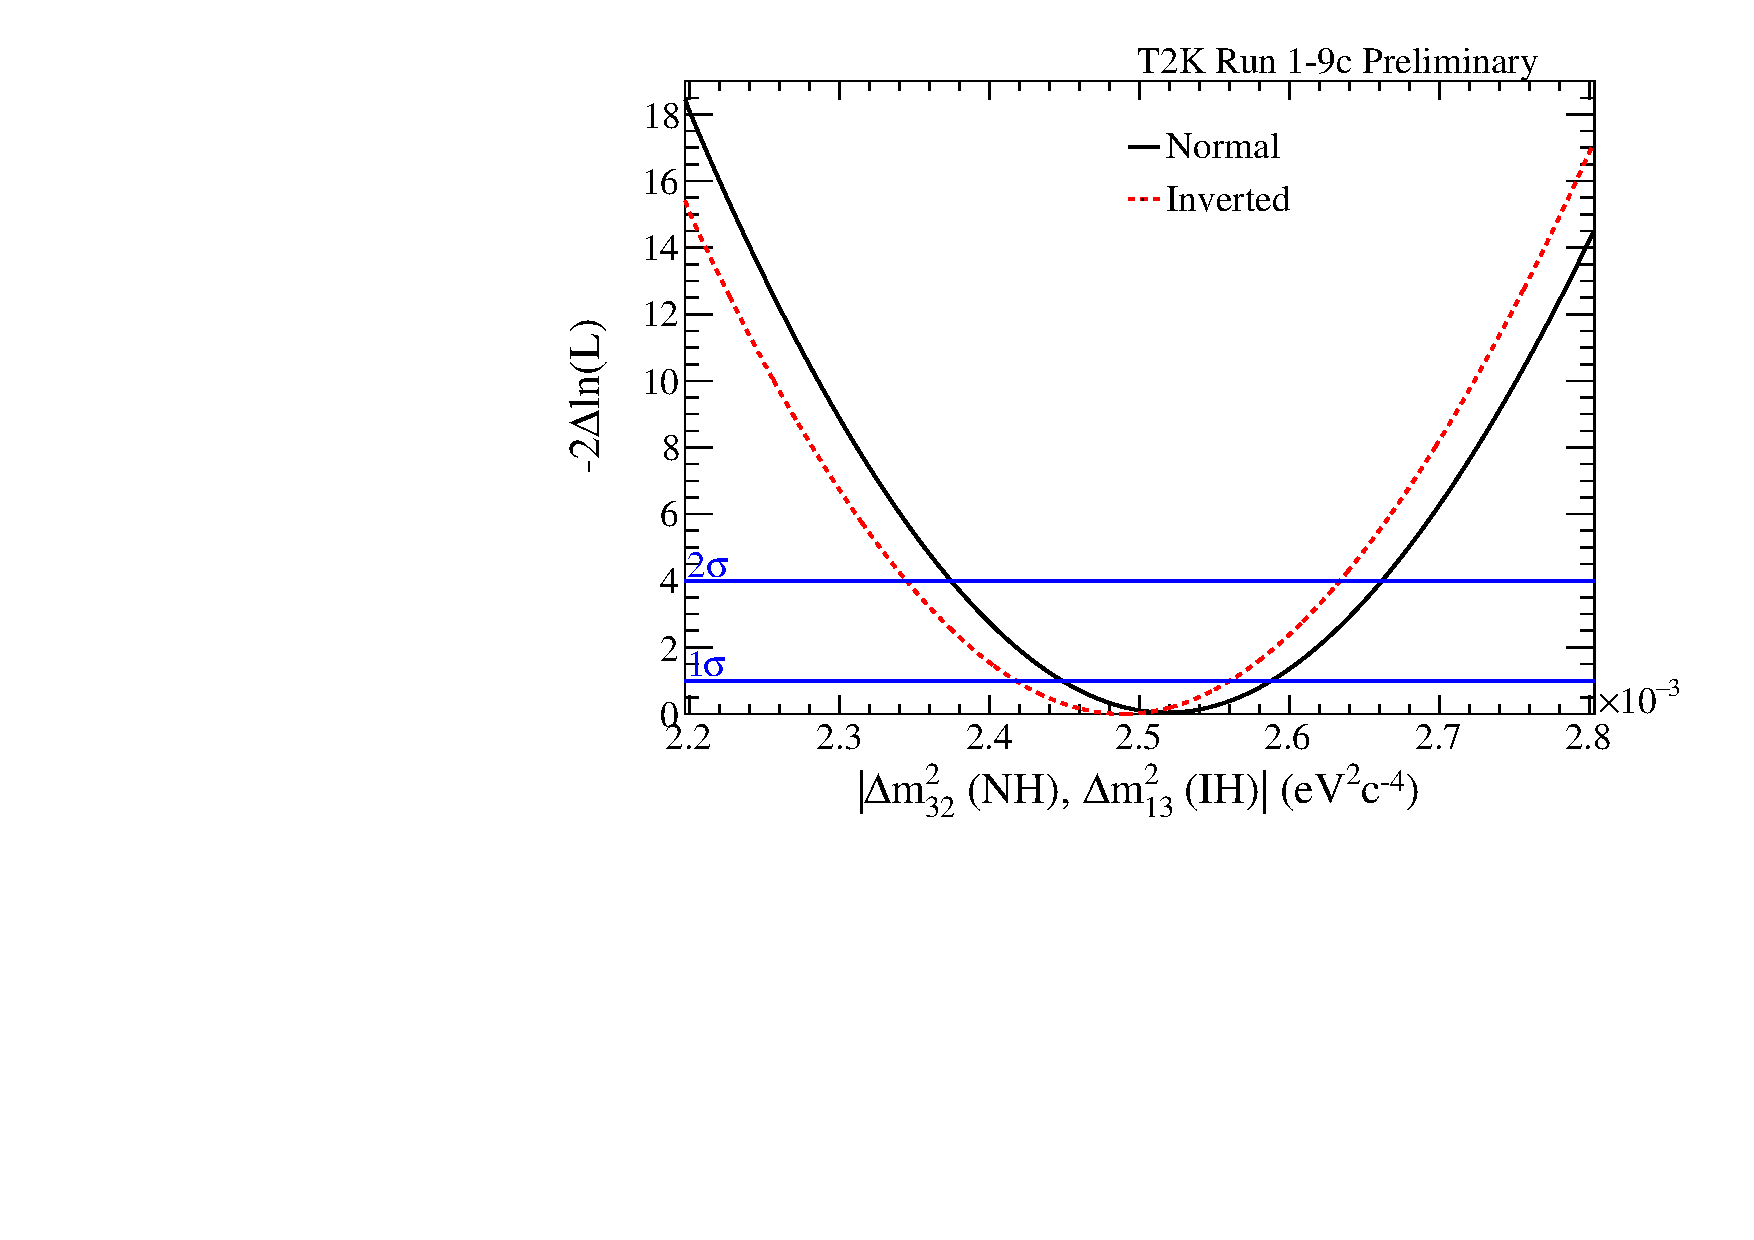
\includegraphics[width=0.9\textwidth]{images/sensitivity/dmsq23_AsimovB_reactor_global}
		\caption{Asimov B \dmsq with reactor constraint}
	\end{subfigure}
	\begin{subfigure}[b]{0.49\textwidth}
		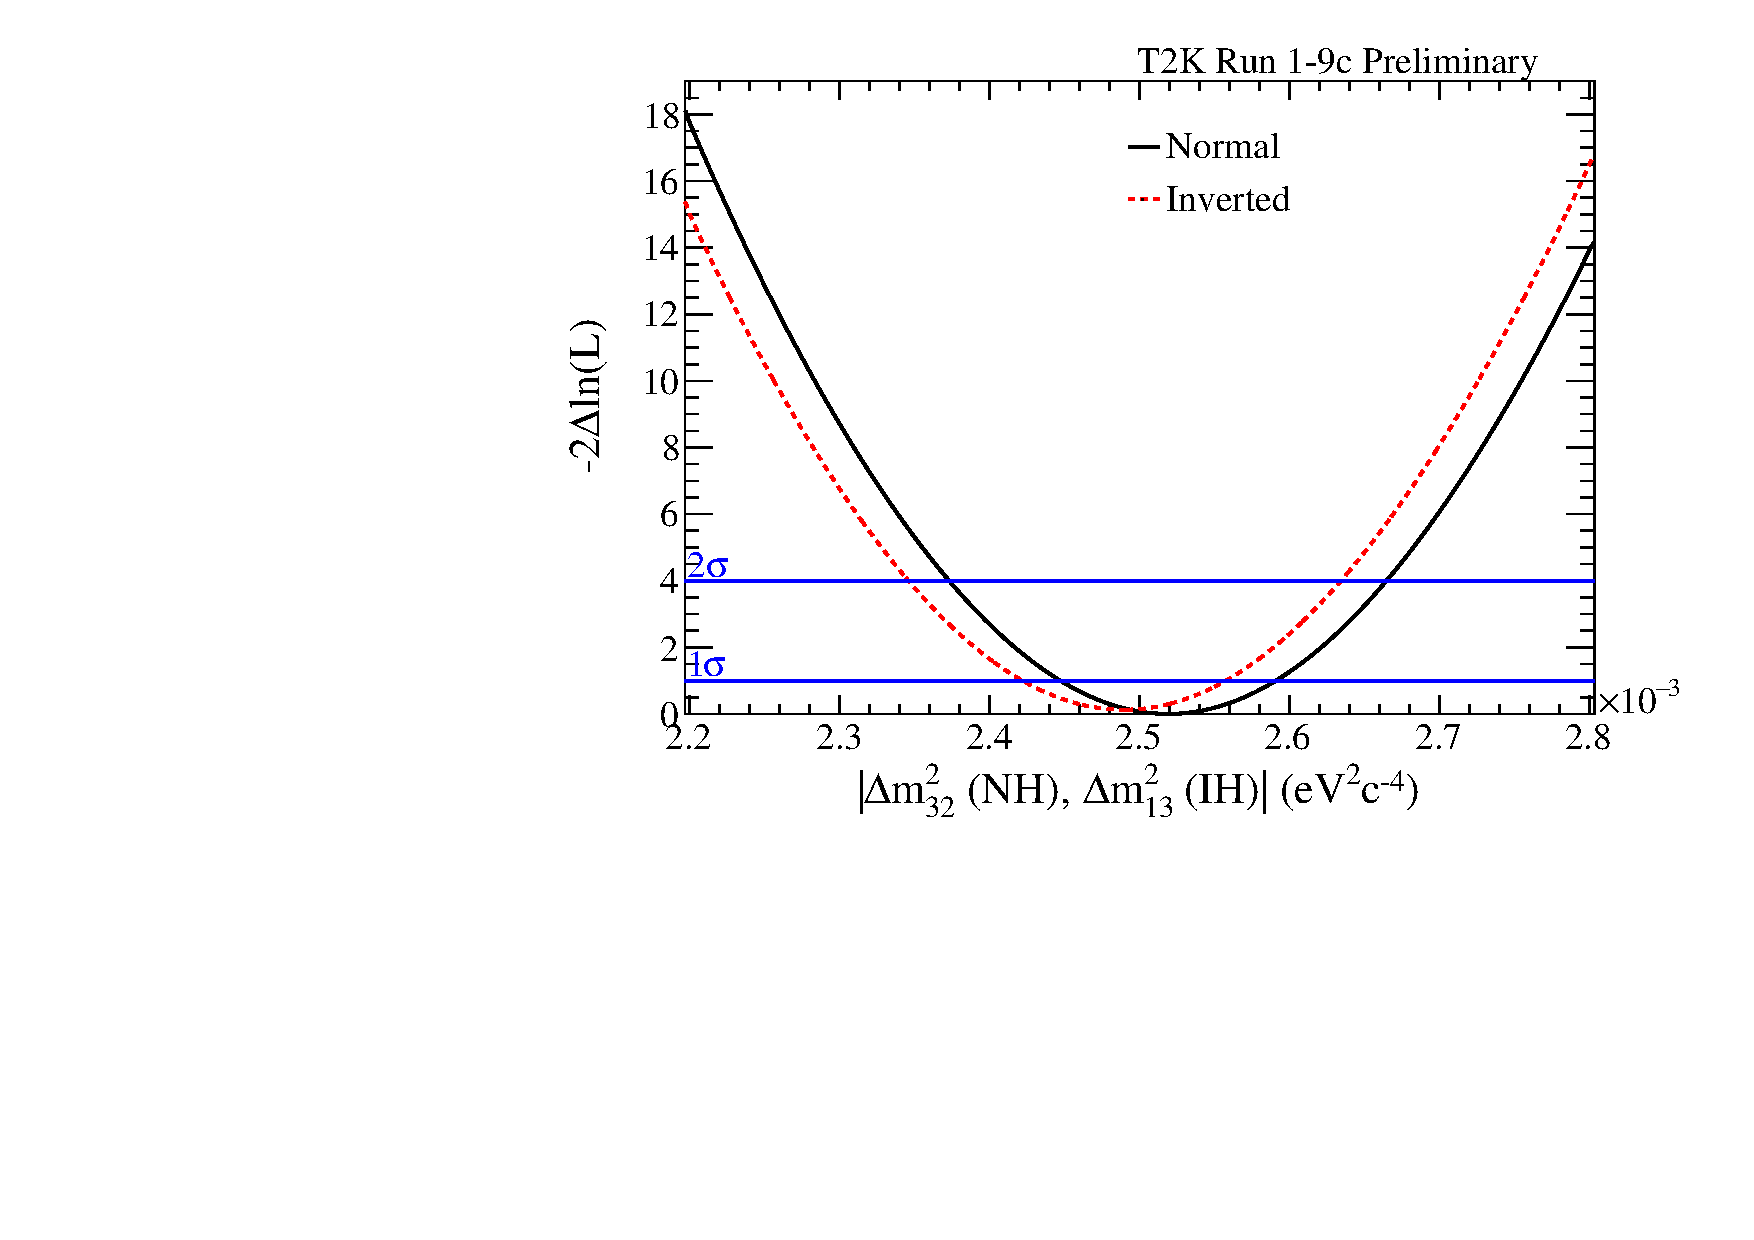
\includegraphics[width=0.9\textwidth]{images/sensitivity/dmsq23_AsimovB_t2k_global}
		\caption{Asimov B \dmsq T2K only}
	\end{subfigure}
	\caption {
		The expected $\Delta\chi^2$ distribution as a function of \dmsq with and without reactor constraint for Asimov data sets A and B. The mass hierarchy is minimized, with normal and inverted hierarchy $\Delta\chi^2$ distributions shifted to the same global best-fit $\chi^2$ value, which is taken to be the minimum between normal and inverted hierarchy. All 5 samples were used to produce these fits.
	}
	\label{fig:dmsq23_sensitivity}
\end{figure*}
